% Options for packages loaded elsewhere
\PassOptionsToPackage{unicode}{hyperref}
\PassOptionsToPackage{hyphens}{url}
\PassOptionsToPackage{dvipsnames,svgnames,x11names}{xcolor}
%
\documentclass[
  letterpaper,
  DIV=11,
  numbers=noendperiod]{scrartcl}

\usepackage{amsmath,amssymb}
\usepackage{iftex}
\ifPDFTeX
  \usepackage[T1]{fontenc}
  \usepackage[utf8]{inputenc}
  \usepackage{textcomp} % provide euro and other symbols
\else % if luatex or xetex
  \usepackage{unicode-math}
  \defaultfontfeatures{Scale=MatchLowercase}
  \defaultfontfeatures[\rmfamily]{Ligatures=TeX,Scale=1}
\fi
\usepackage{lmodern}
\ifPDFTeX\else  
    % xetex/luatex font selection
\fi
% Use upquote if available, for straight quotes in verbatim environments
\IfFileExists{upquote.sty}{\usepackage{upquote}}{}
\IfFileExists{microtype.sty}{% use microtype if available
  \usepackage[]{microtype}
  \UseMicrotypeSet[protrusion]{basicmath} % disable protrusion for tt fonts
}{}
\makeatletter
\@ifundefined{KOMAClassName}{% if non-KOMA class
  \IfFileExists{parskip.sty}{%
    \usepackage{parskip}
  }{% else
    \setlength{\parindent}{0pt}
    \setlength{\parskip}{6pt plus 2pt minus 1pt}}
}{% if KOMA class
  \KOMAoptions{parskip=half}}
\makeatother
\usepackage{xcolor}
\usepackage[top=10mm,bottom=2mm]{geometry}
\setlength{\emergencystretch}{3em} % prevent overfull lines
\setcounter{secnumdepth}{-\maxdimen} % remove section numbering
% Make \paragraph and \subparagraph free-standing
\ifx\paragraph\undefined\else
  \let\oldparagraph\paragraph
  \renewcommand{\paragraph}[1]{\oldparagraph{#1}\mbox{}}
\fi
\ifx\subparagraph\undefined\else
  \let\oldsubparagraph\subparagraph
  \renewcommand{\subparagraph}[1]{\oldsubparagraph{#1}\mbox{}}
\fi


\providecommand{\tightlist}{%
  \setlength{\itemsep}{0pt}\setlength{\parskip}{0pt}}\usepackage{longtable,booktabs,array}
\usepackage{calc} % for calculating minipage widths
% Correct order of tables after \paragraph or \subparagraph
\usepackage{etoolbox}
\makeatletter
\patchcmd\longtable{\par}{\if@noskipsec\mbox{}\fi\par}{}{}
\makeatother
% Allow footnotes in longtable head/foot
\IfFileExists{footnotehyper.sty}{\usepackage{footnotehyper}}{\usepackage{footnote}}
\makesavenoteenv{longtable}
\usepackage{graphicx}
\makeatletter
\def\maxwidth{\ifdim\Gin@nat@width>\linewidth\linewidth\else\Gin@nat@width\fi}
\def\maxheight{\ifdim\Gin@nat@height>\textheight\textheight\else\Gin@nat@height\fi}
\makeatother
% Scale images if necessary, so that they will not overflow the page
% margins by default, and it is still possible to overwrite the defaults
% using explicit options in \includegraphics[width, height, ...]{}
\setkeys{Gin}{width=\maxwidth,height=\maxheight,keepaspectratio}
% Set default figure placement to htbp
\makeatletter
\def\fps@figure{htbp}
\makeatother

\usepackage{booktabs}
\usepackage{longtable}
\usepackage{array}
\usepackage{multirow}
\usepackage{wrapfig}
\usepackage{float}
\usepackage{colortbl}
\usepackage{pdflscape}
\usepackage{tabu}
\usepackage{threeparttable}
\usepackage{threeparttablex}
\usepackage[normalem]{ulem}
\usepackage{makecell}
\usepackage{xcolor}
\usepackage{typearea}
\KOMAoption{captions}{tableheading}
\makeatletter
\makeatother
\makeatletter
\makeatother
\makeatletter
\@ifpackageloaded{caption}{}{\usepackage{caption}}
\AtBeginDocument{%
\ifdefined\contentsname
  \renewcommand*\contentsname{Table of contents}
\else
  \newcommand\contentsname{Table of contents}
\fi
\ifdefined\listfigurename
  \renewcommand*\listfigurename{List of Figures}
\else
  \newcommand\listfigurename{List of Figures}
\fi
\ifdefined\listtablename
  \renewcommand*\listtablename{List of Tables}
\else
  \newcommand\listtablename{List of Tables}
\fi
\ifdefined\figurename
  \renewcommand*\figurename{Figure}
\else
  \newcommand\figurename{Figure}
\fi
\ifdefined\tablename
  \renewcommand*\tablename{Table}
\else
  \newcommand\tablename{Table}
\fi
}
\@ifpackageloaded{float}{}{\usepackage{float}}
\floatstyle{ruled}
\@ifundefined{c@chapter}{\newfloat{codelisting}{h}{lop}}{\newfloat{codelisting}{h}{lop}[chapter]}
\floatname{codelisting}{Listing}
\newcommand*\listoflistings{\listof{codelisting}{List of Listings}}
\makeatother
\makeatletter
\@ifpackageloaded{caption}{}{\usepackage{caption}}
\@ifpackageloaded{subcaption}{}{\usepackage{subcaption}}
\makeatother
\makeatletter
\@ifpackageloaded{tcolorbox}{}{\usepackage[skins,breakable]{tcolorbox}}
\makeatother
\makeatletter
\@ifundefined{shadecolor}{\definecolor{shadecolor}{rgb}{.97, .97, .97}}
\makeatother
\makeatletter
\makeatother
\makeatletter
\makeatother
\ifLuaTeX
  \usepackage{selnolig}  % disable illegal ligatures
\fi
\IfFileExists{bookmark.sty}{\usepackage{bookmark}}{\usepackage{hyperref}}
\IfFileExists{xurl.sty}{\usepackage{xurl}}{} % add URL line breaks if available
\urlstyle{same} % disable monospaced font for URLs
\hypersetup{
  pdftitle={Simulation Result},
  pdfauthor={Shafayet Khan Shafee},
  colorlinks=true,
  linkcolor={blue},
  filecolor={Maroon},
  citecolor={Blue},
  urlcolor={Blue},
  pdfcreator={LaTeX via pandoc}}

\title{Simulation Result}
\author{Shafayet Khan Shafee}
\date{05 August 2023}

\begin{document}
\maketitle
\ifdefined\Shaded\renewenvironment{Shaded}{\begin{tcolorbox}[interior hidden, boxrule=0pt, breakable, frame hidden, enhanced, sharp corners, borderline west={3pt}{0pt}{shadecolor}]}{\end{tcolorbox}}\fi

\hypertarget{histograms-for-logwidehatmor-when-cluster-size-is-10}{%
\section{\texorpdfstring{Histograms for \(log(\widehat{MOR})\) When
Cluster Size is
10}{Histograms for log(\textbackslash widehat\{MOR\}) When Cluster Size is 10}}\label{histograms-for-logwidehatmor-when-cluster-size-is-10}}

\vspace{5mm}

\begin{figure}

\begin{minipage}[t]{0.44\linewidth}

{\centering 

\raisebox{-\height}{

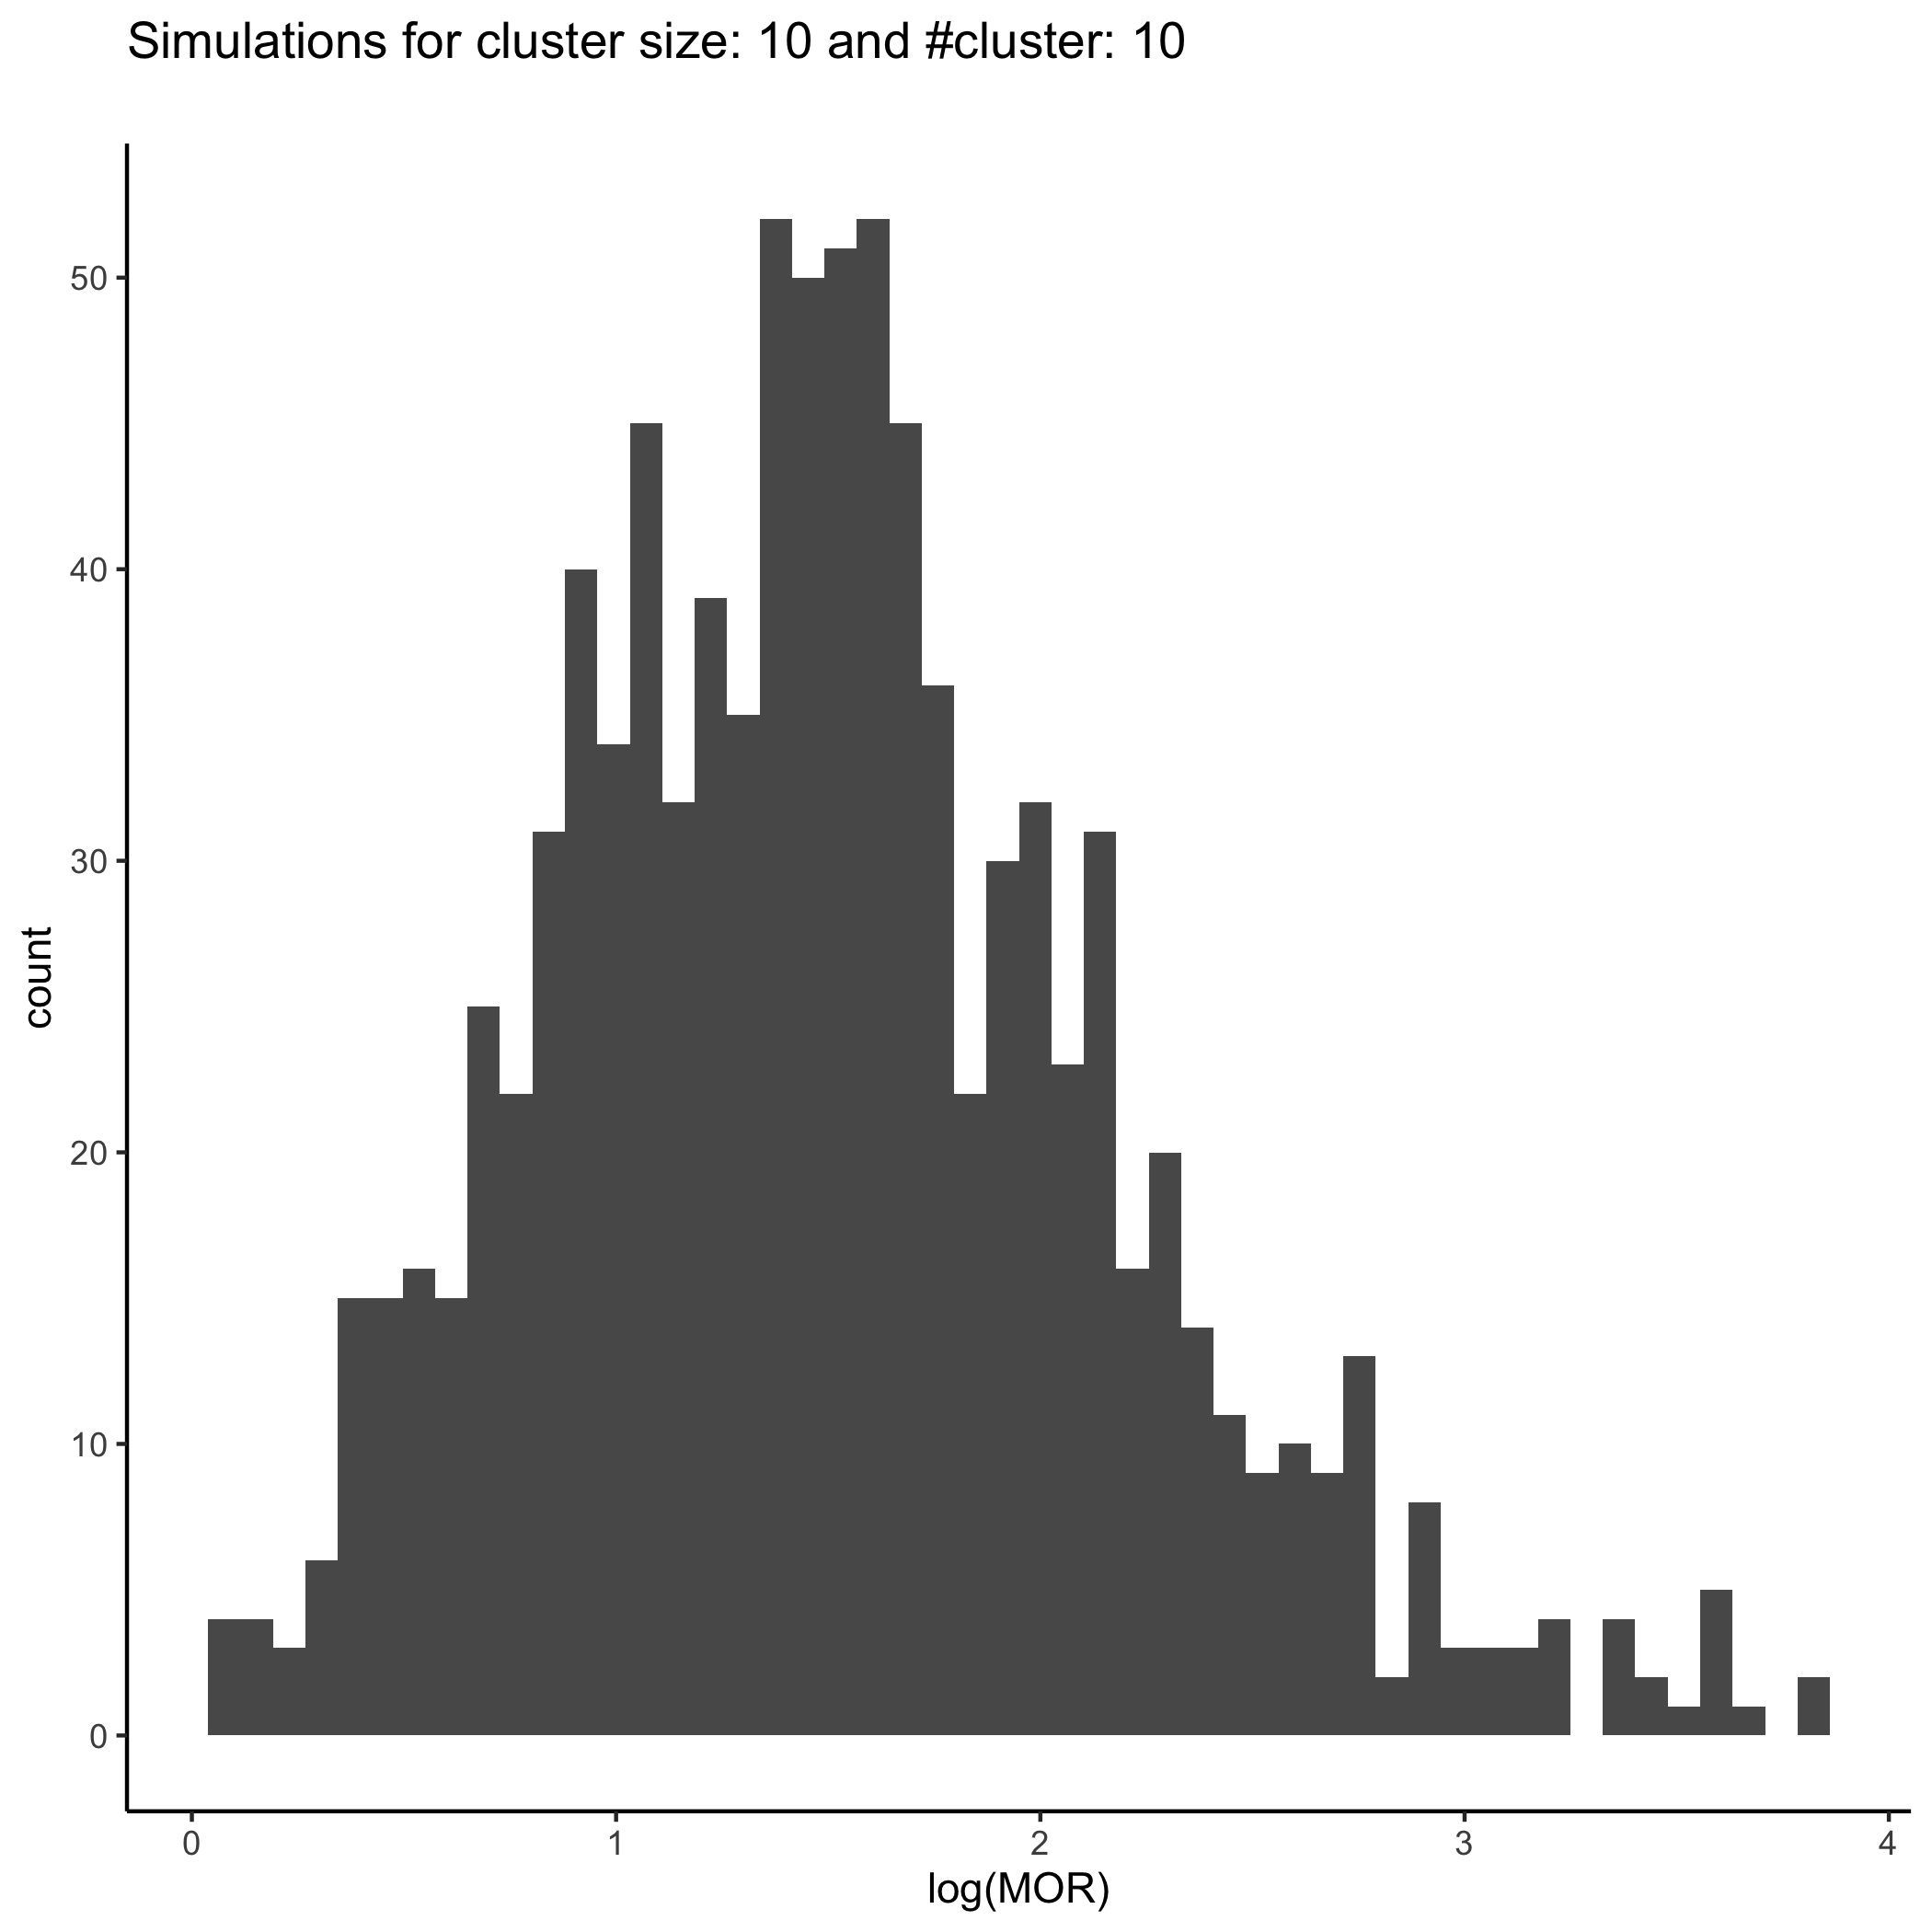
\includegraphics{../plots/hist_10_10.png}

}

\caption{For 10 clusters when each of the cluster size is 10}

}

\end{minipage}%
%
\begin{minipage}[t]{0.11\linewidth}

{\centering 

~

}

\end{minipage}%
%
\begin{minipage}[t]{0.44\linewidth}

{\centering 

\raisebox{-\height}{

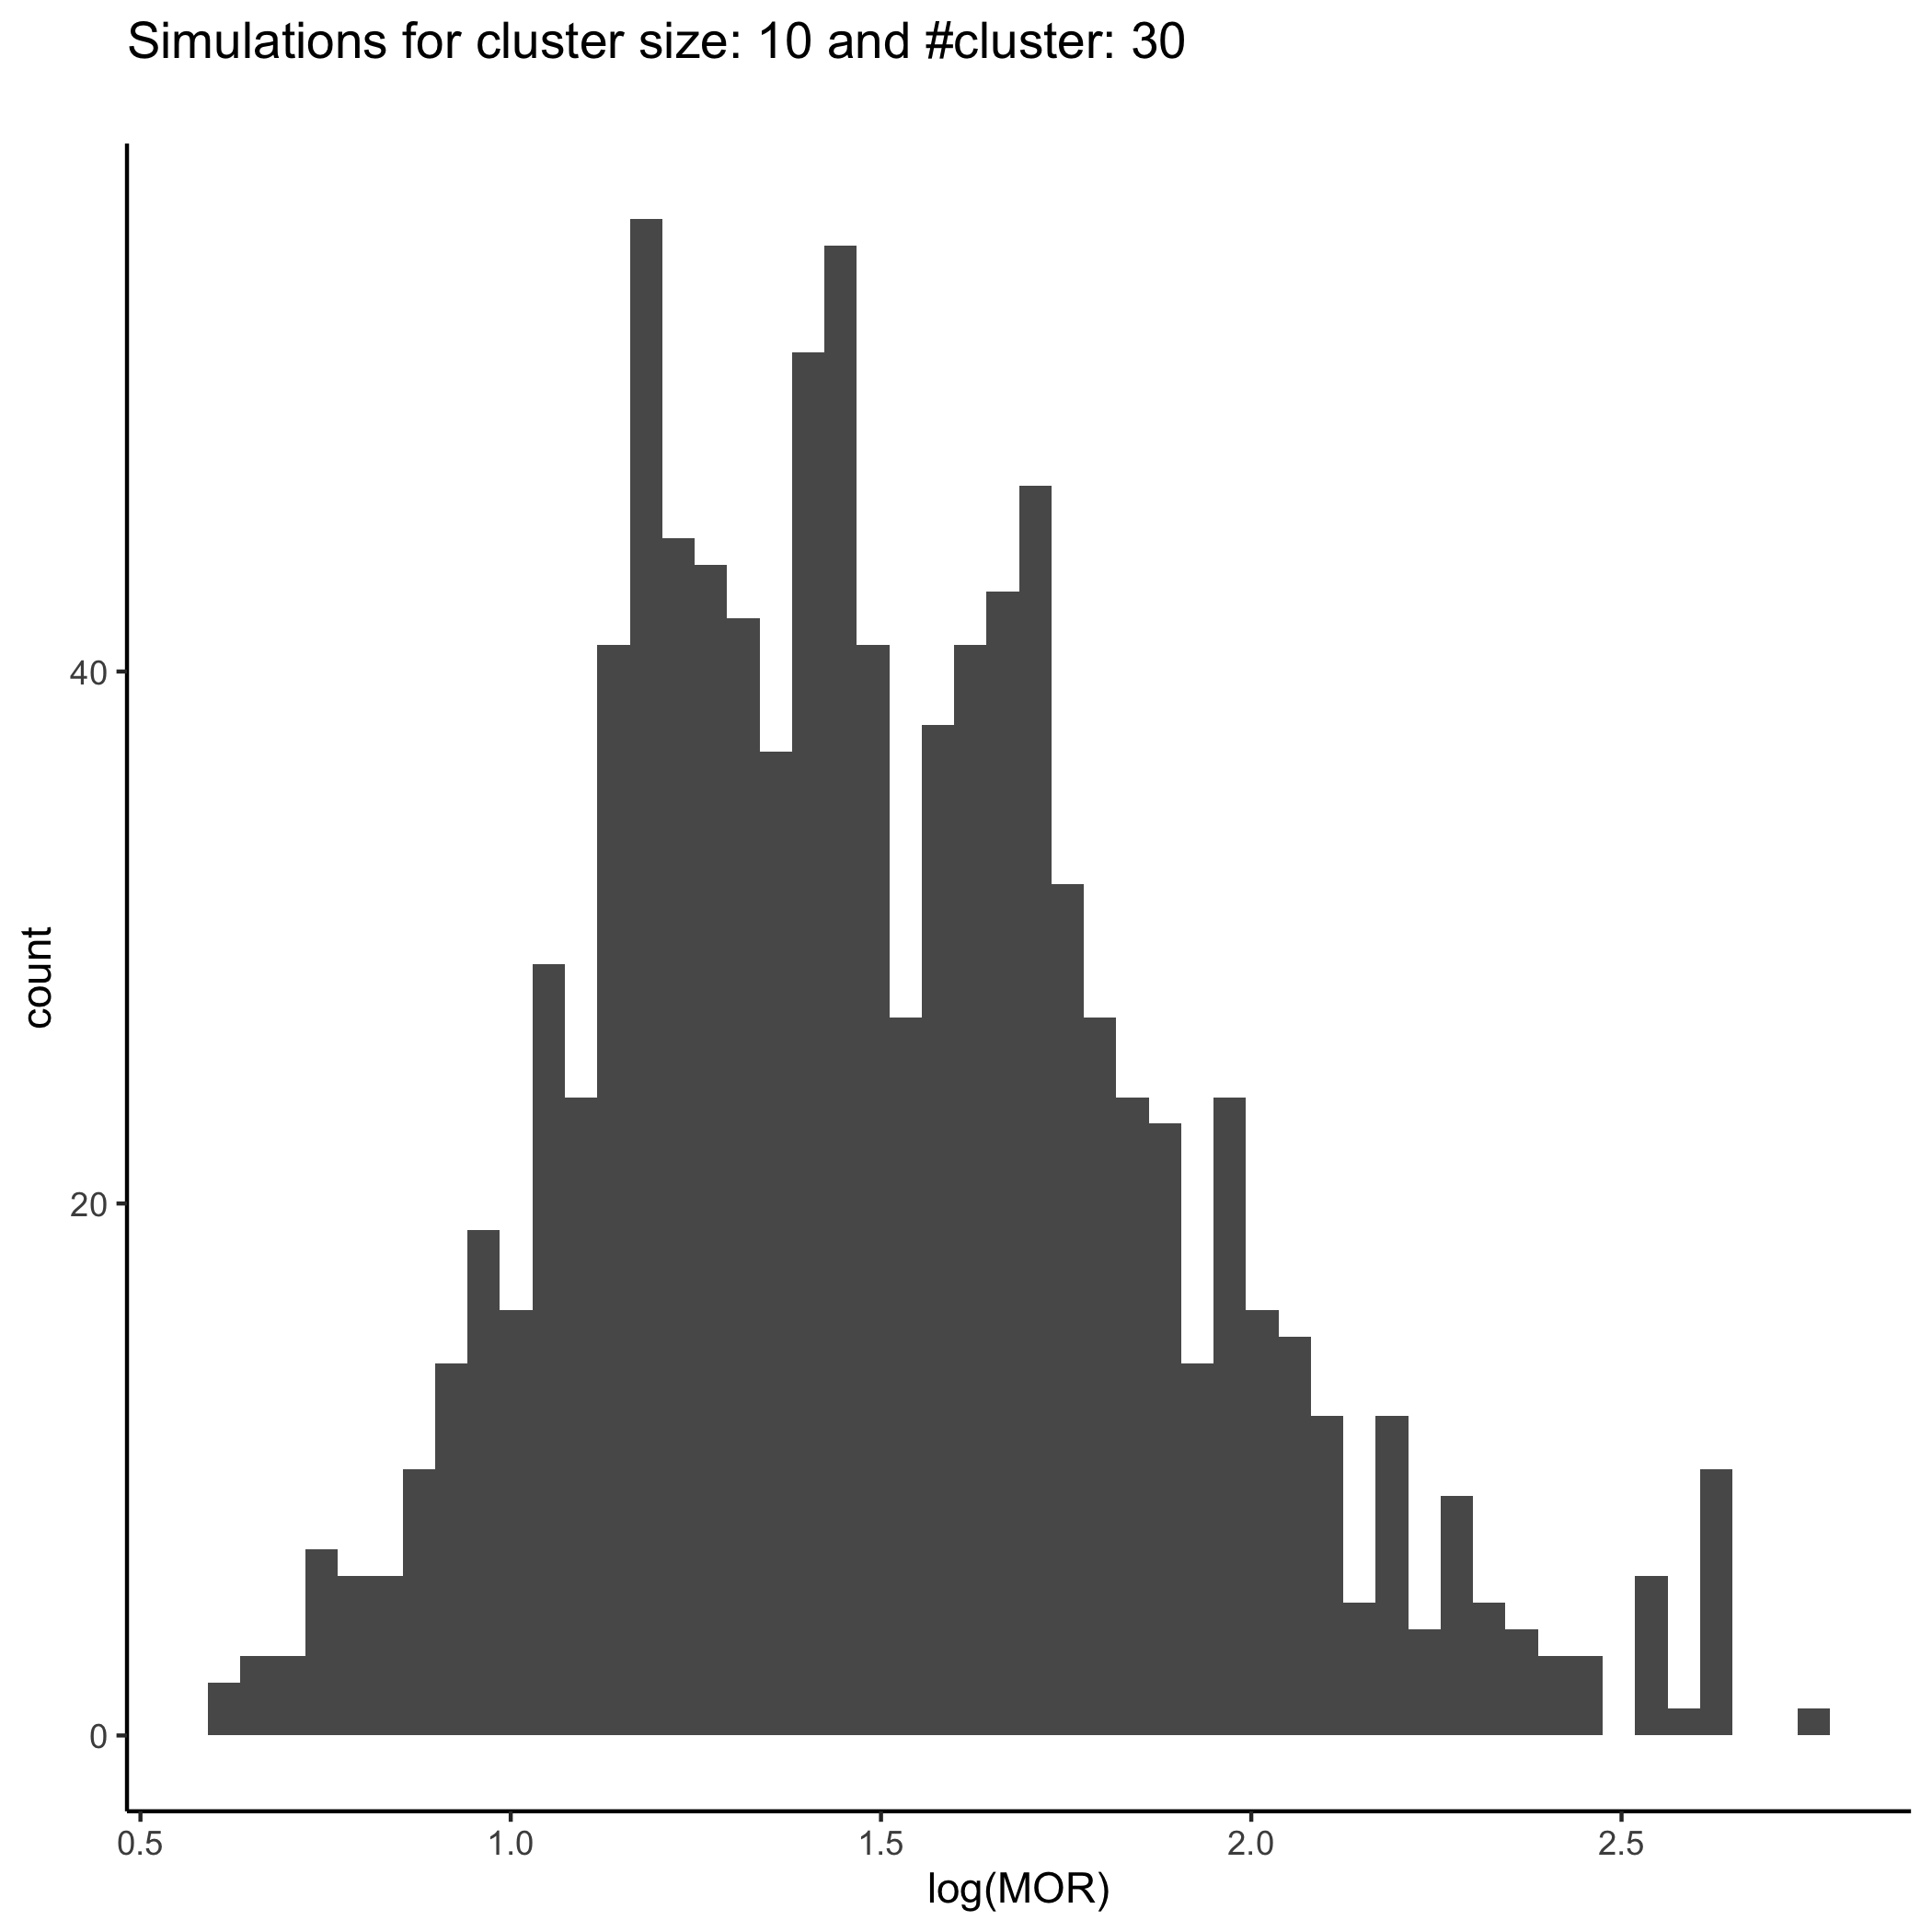
\includegraphics{../plots/hist_30_10.png}

}

\caption{For 30 clusters when each of the cluster size is 10}

}

\end{minipage}%

\end{figure}

\vspace{5mm}

\begin{figure}[H]

{\centering 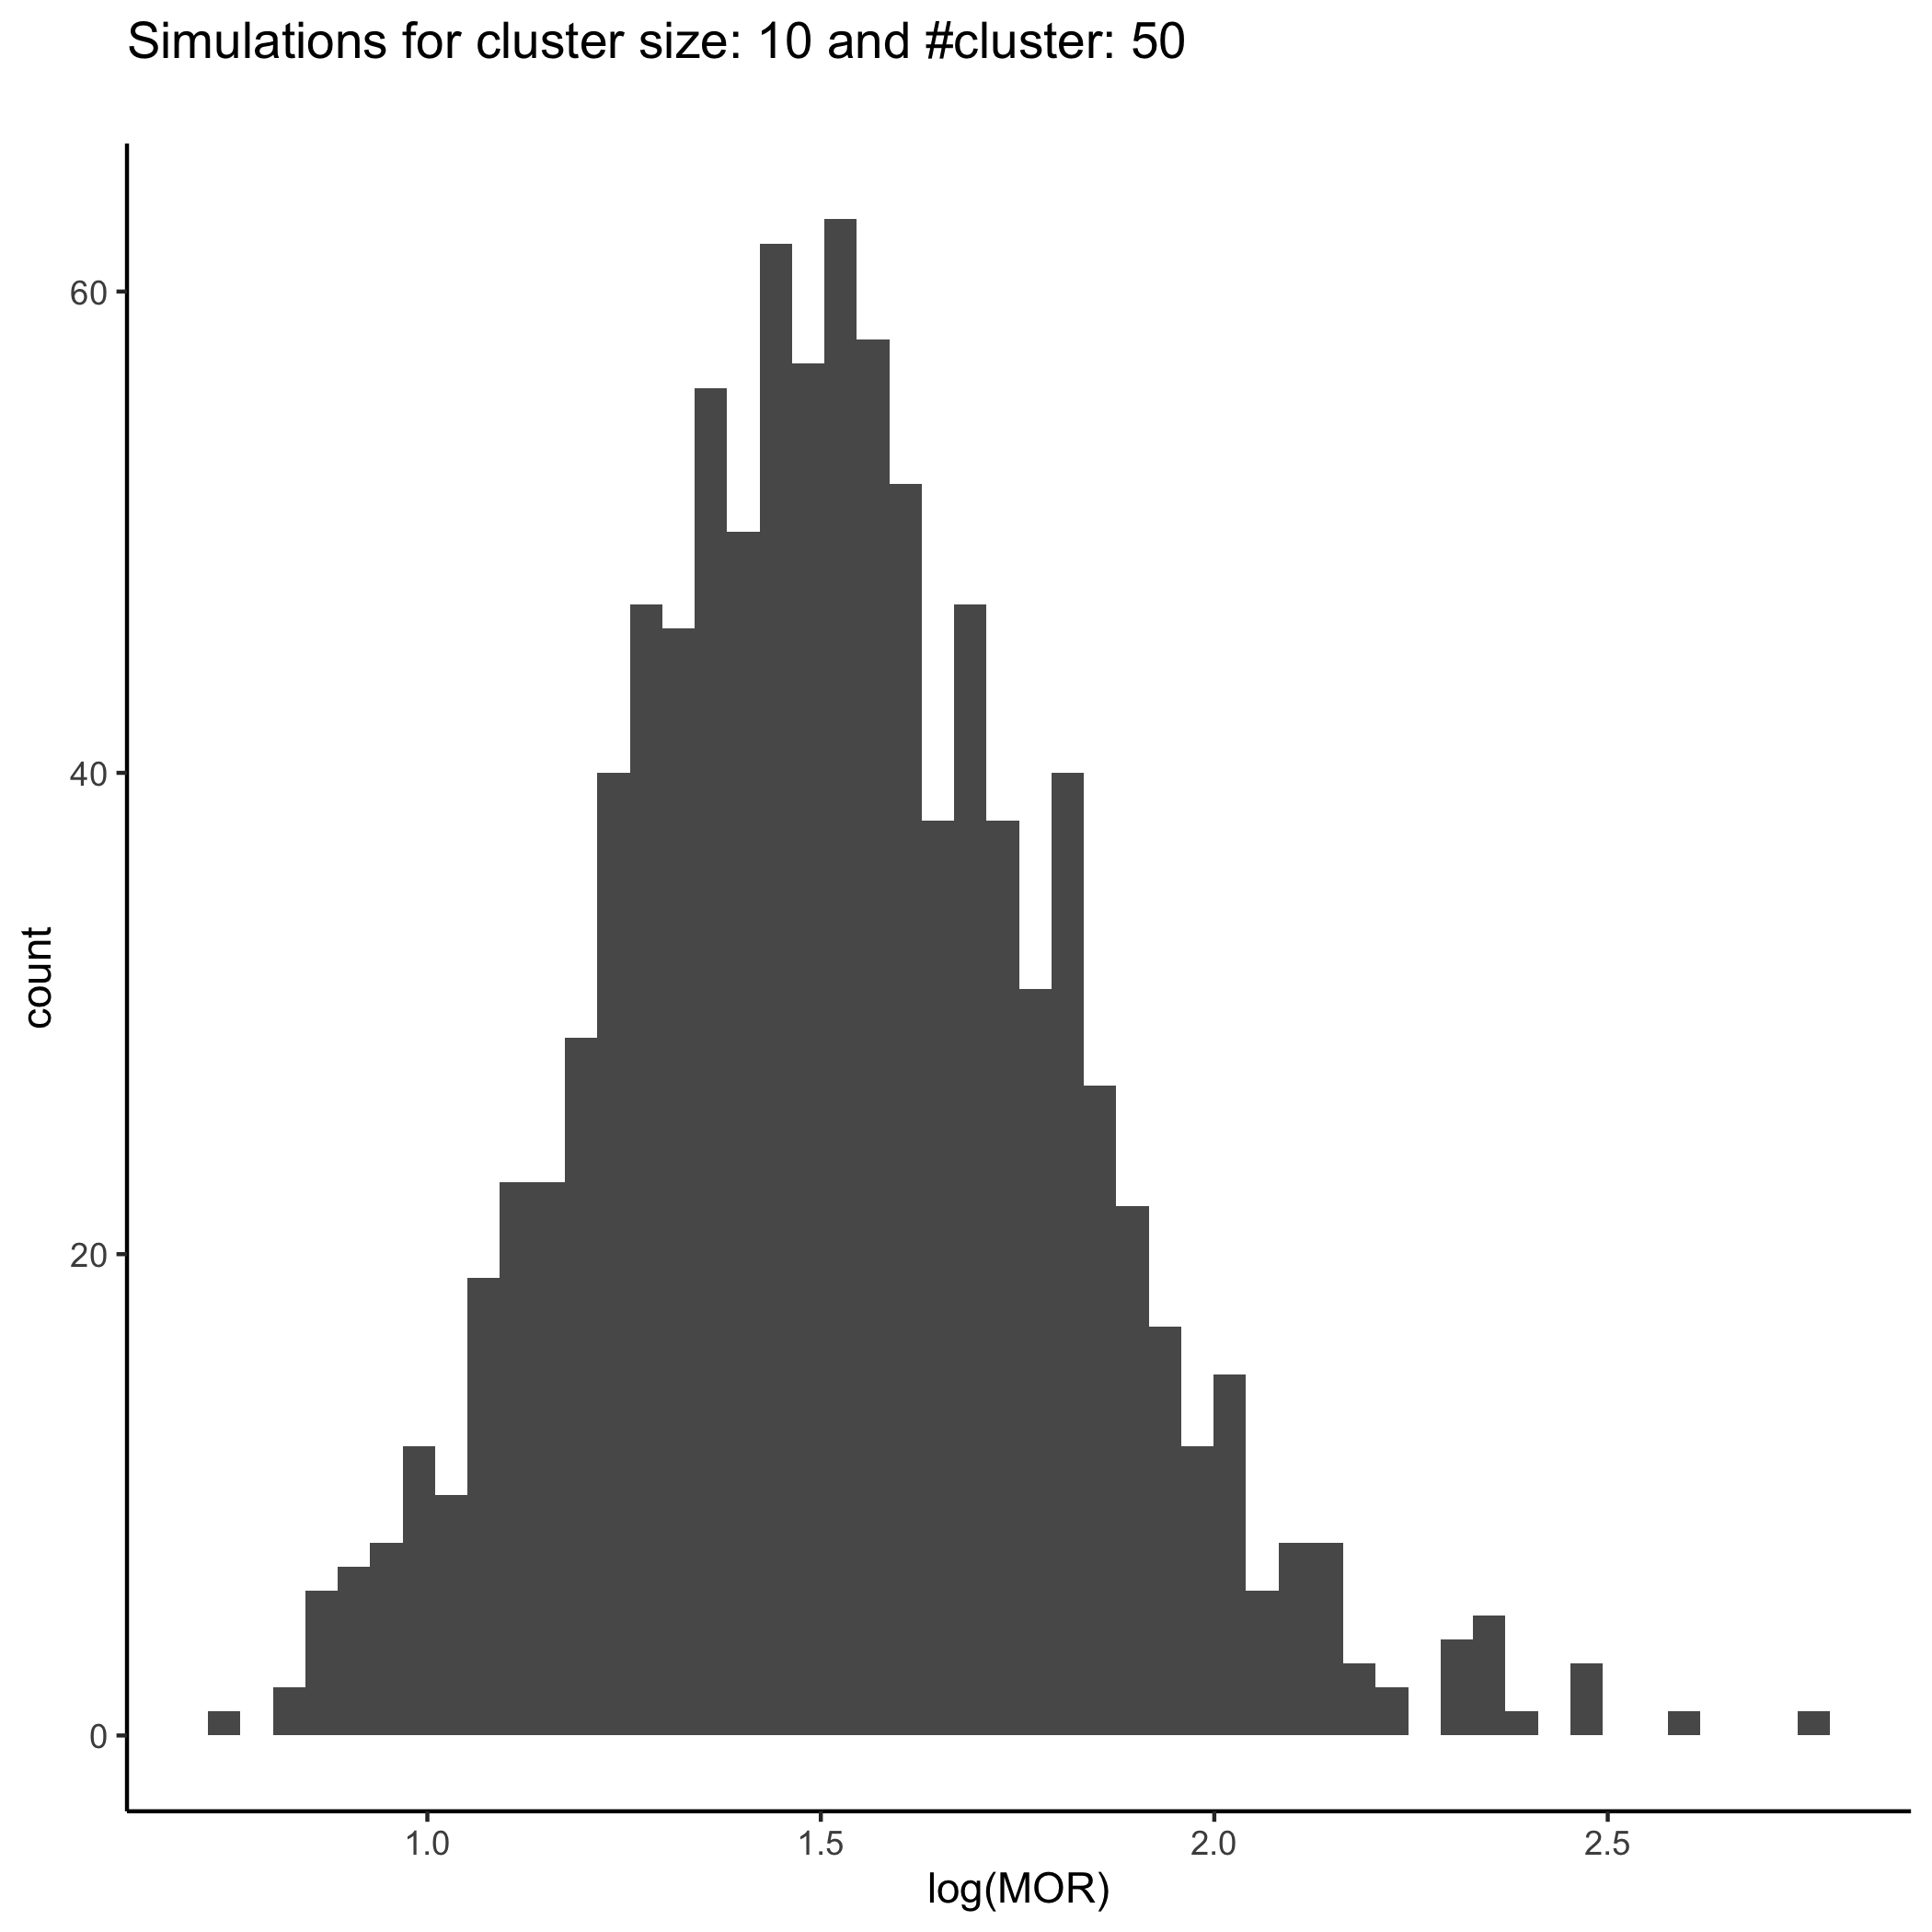
\includegraphics[width=0.5\textwidth,height=\textheight]{../plots/hist_50_10.png}

}

\caption{For 50 clusters when each of the cluster size is 10}

\end{figure}

\newpage

\hypertarget{histograms-for-logwidehatmor-when-cluster-size-is-15}{%
\section{\texorpdfstring{Histograms for \(log(\widehat{MOR})\) When
Cluster Size is
15}{Histograms for log(\textbackslash widehat\{MOR\}) When Cluster Size is 15}}\label{histograms-for-logwidehatmor-when-cluster-size-is-15}}

\vspace{5mm}

\begin{figure}

\begin{minipage}[t]{0.44\linewidth}

{\centering 

\raisebox{-\height}{

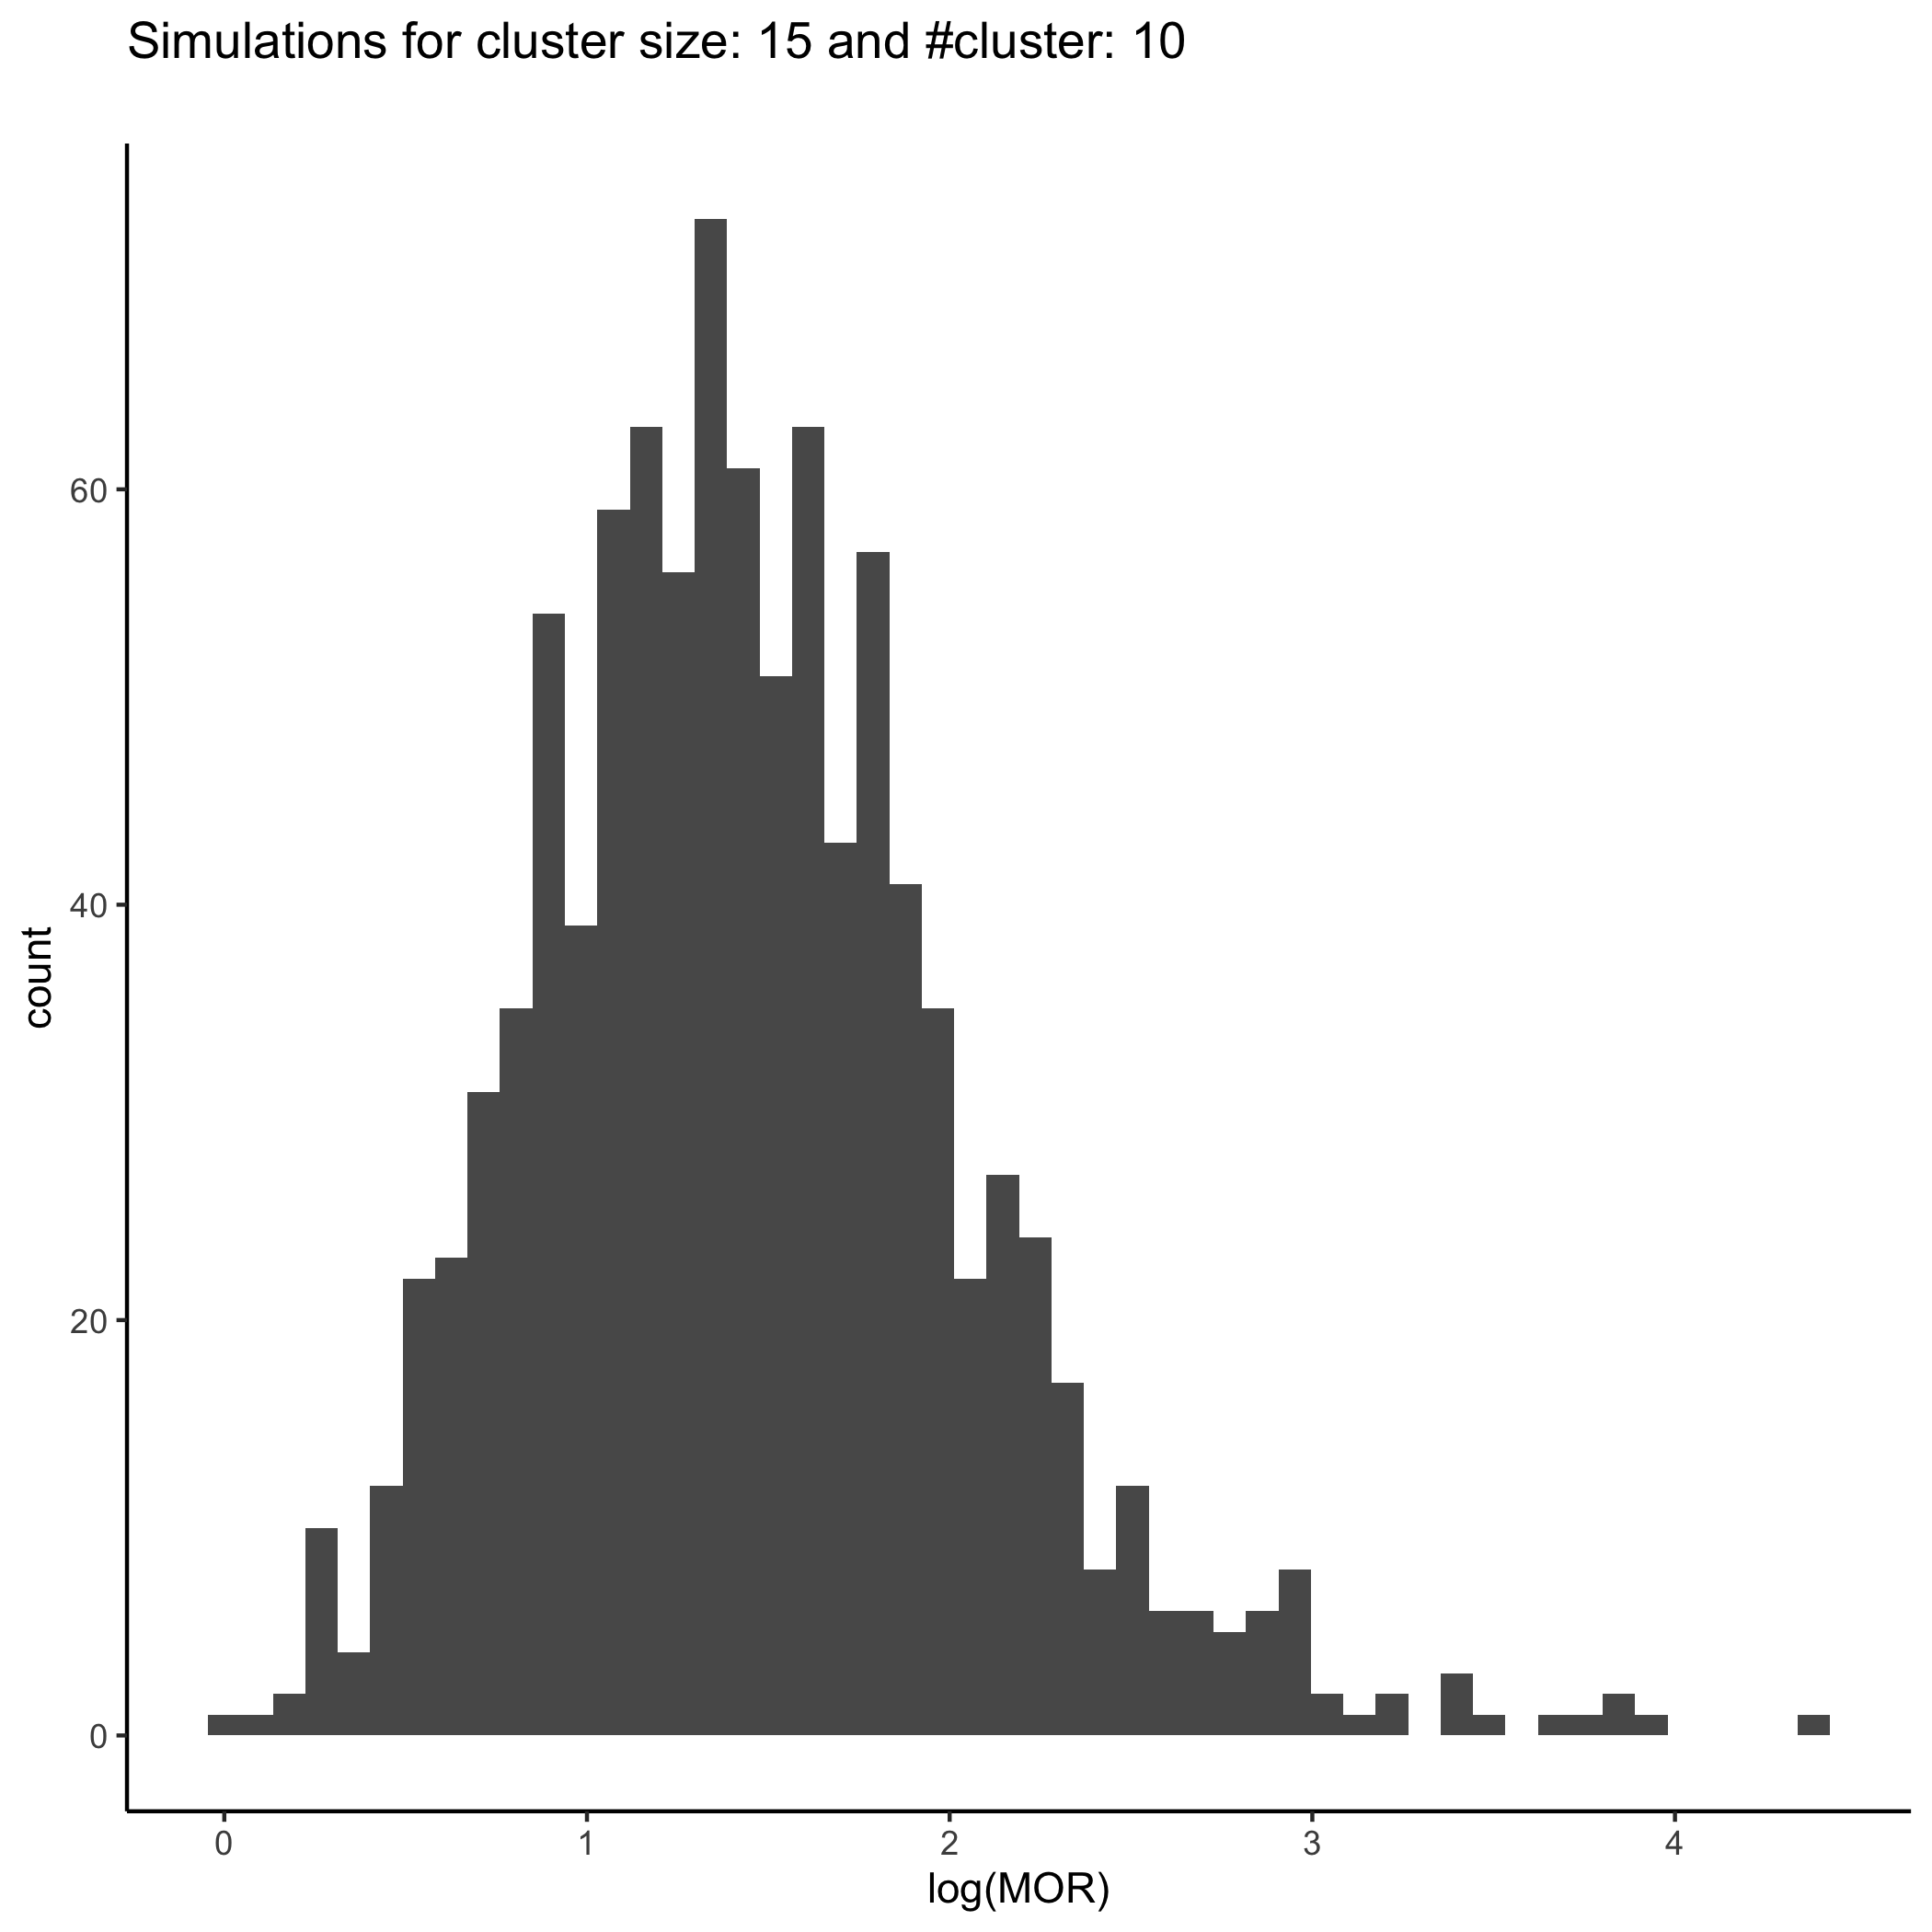
\includegraphics{../plots/hist_10_15.png}

}

\caption{For 10 clusters when each of the cluster size is 115}

}

\end{minipage}%
%
\begin{minipage}[t]{0.11\linewidth}

{\centering 

~

}

\end{minipage}%
%
\begin{minipage}[t]{0.44\linewidth}

{\centering 

\raisebox{-\height}{

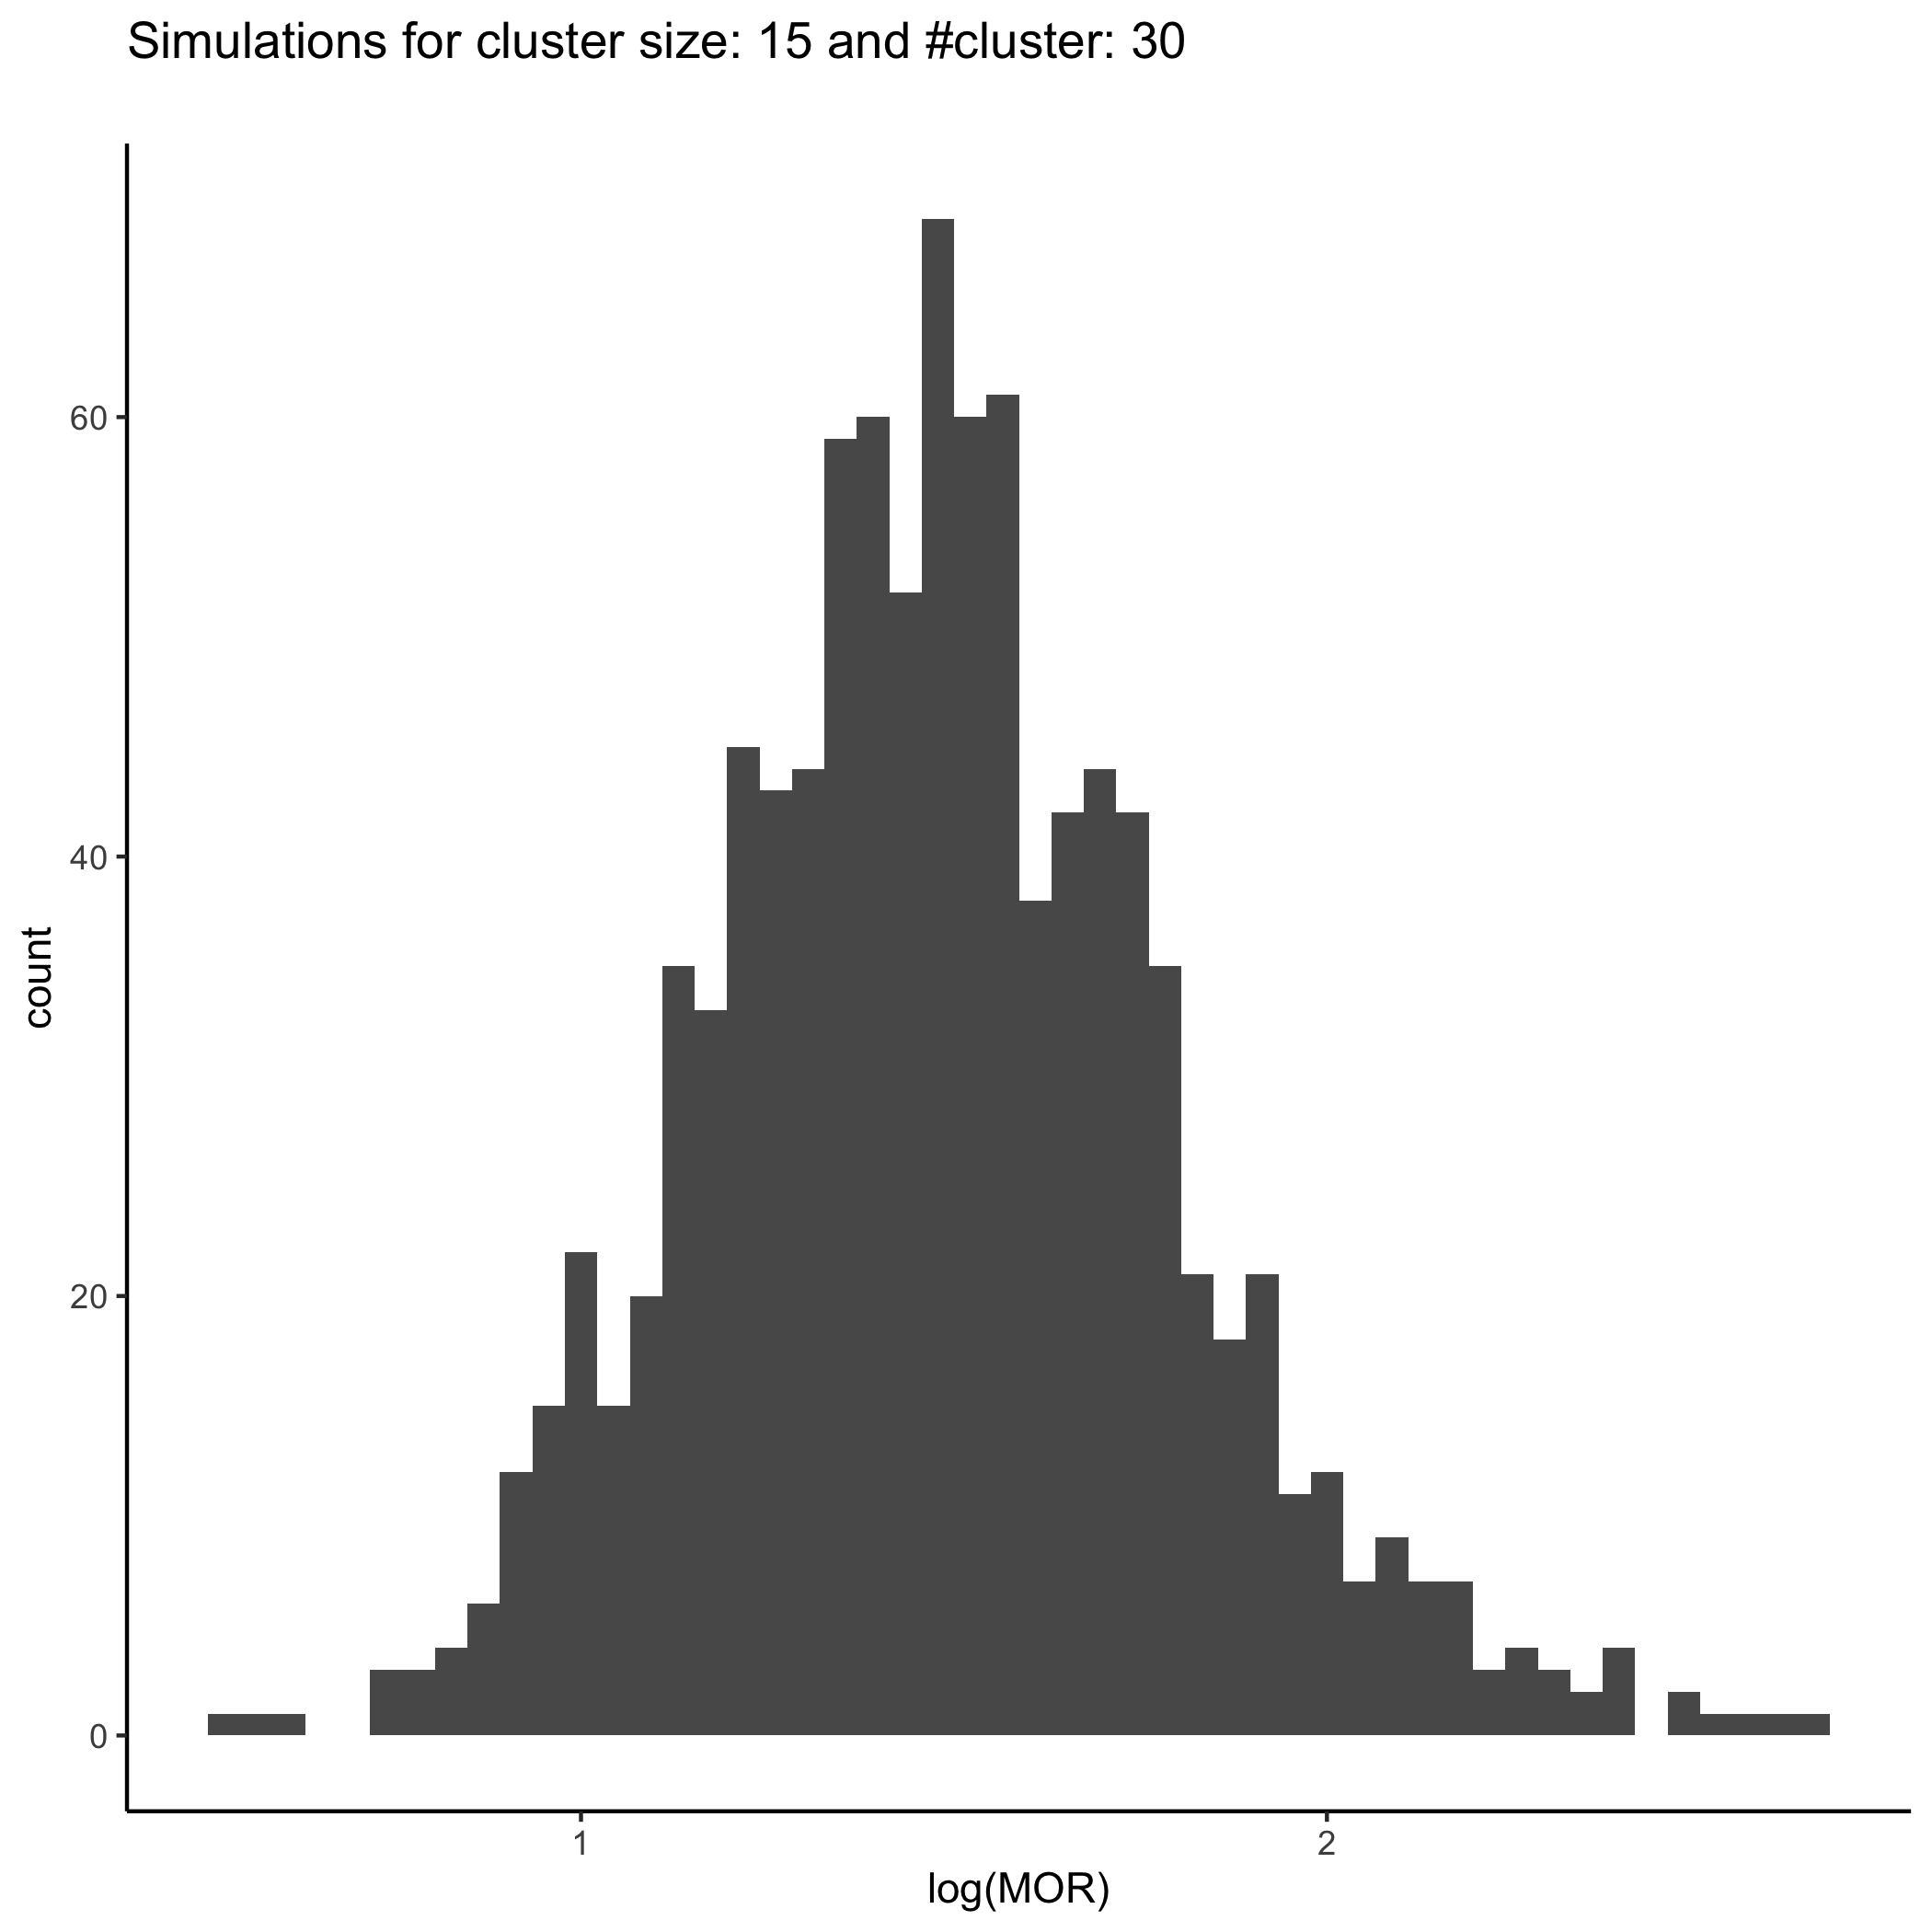
\includegraphics{../plots/hist_30_15.png}

}

\caption{For 30 clusters when each of the cluster size is 15}

}

\end{minipage}%

\end{figure}

\vspace{5mm}

\begin{figure}[H]

{\centering 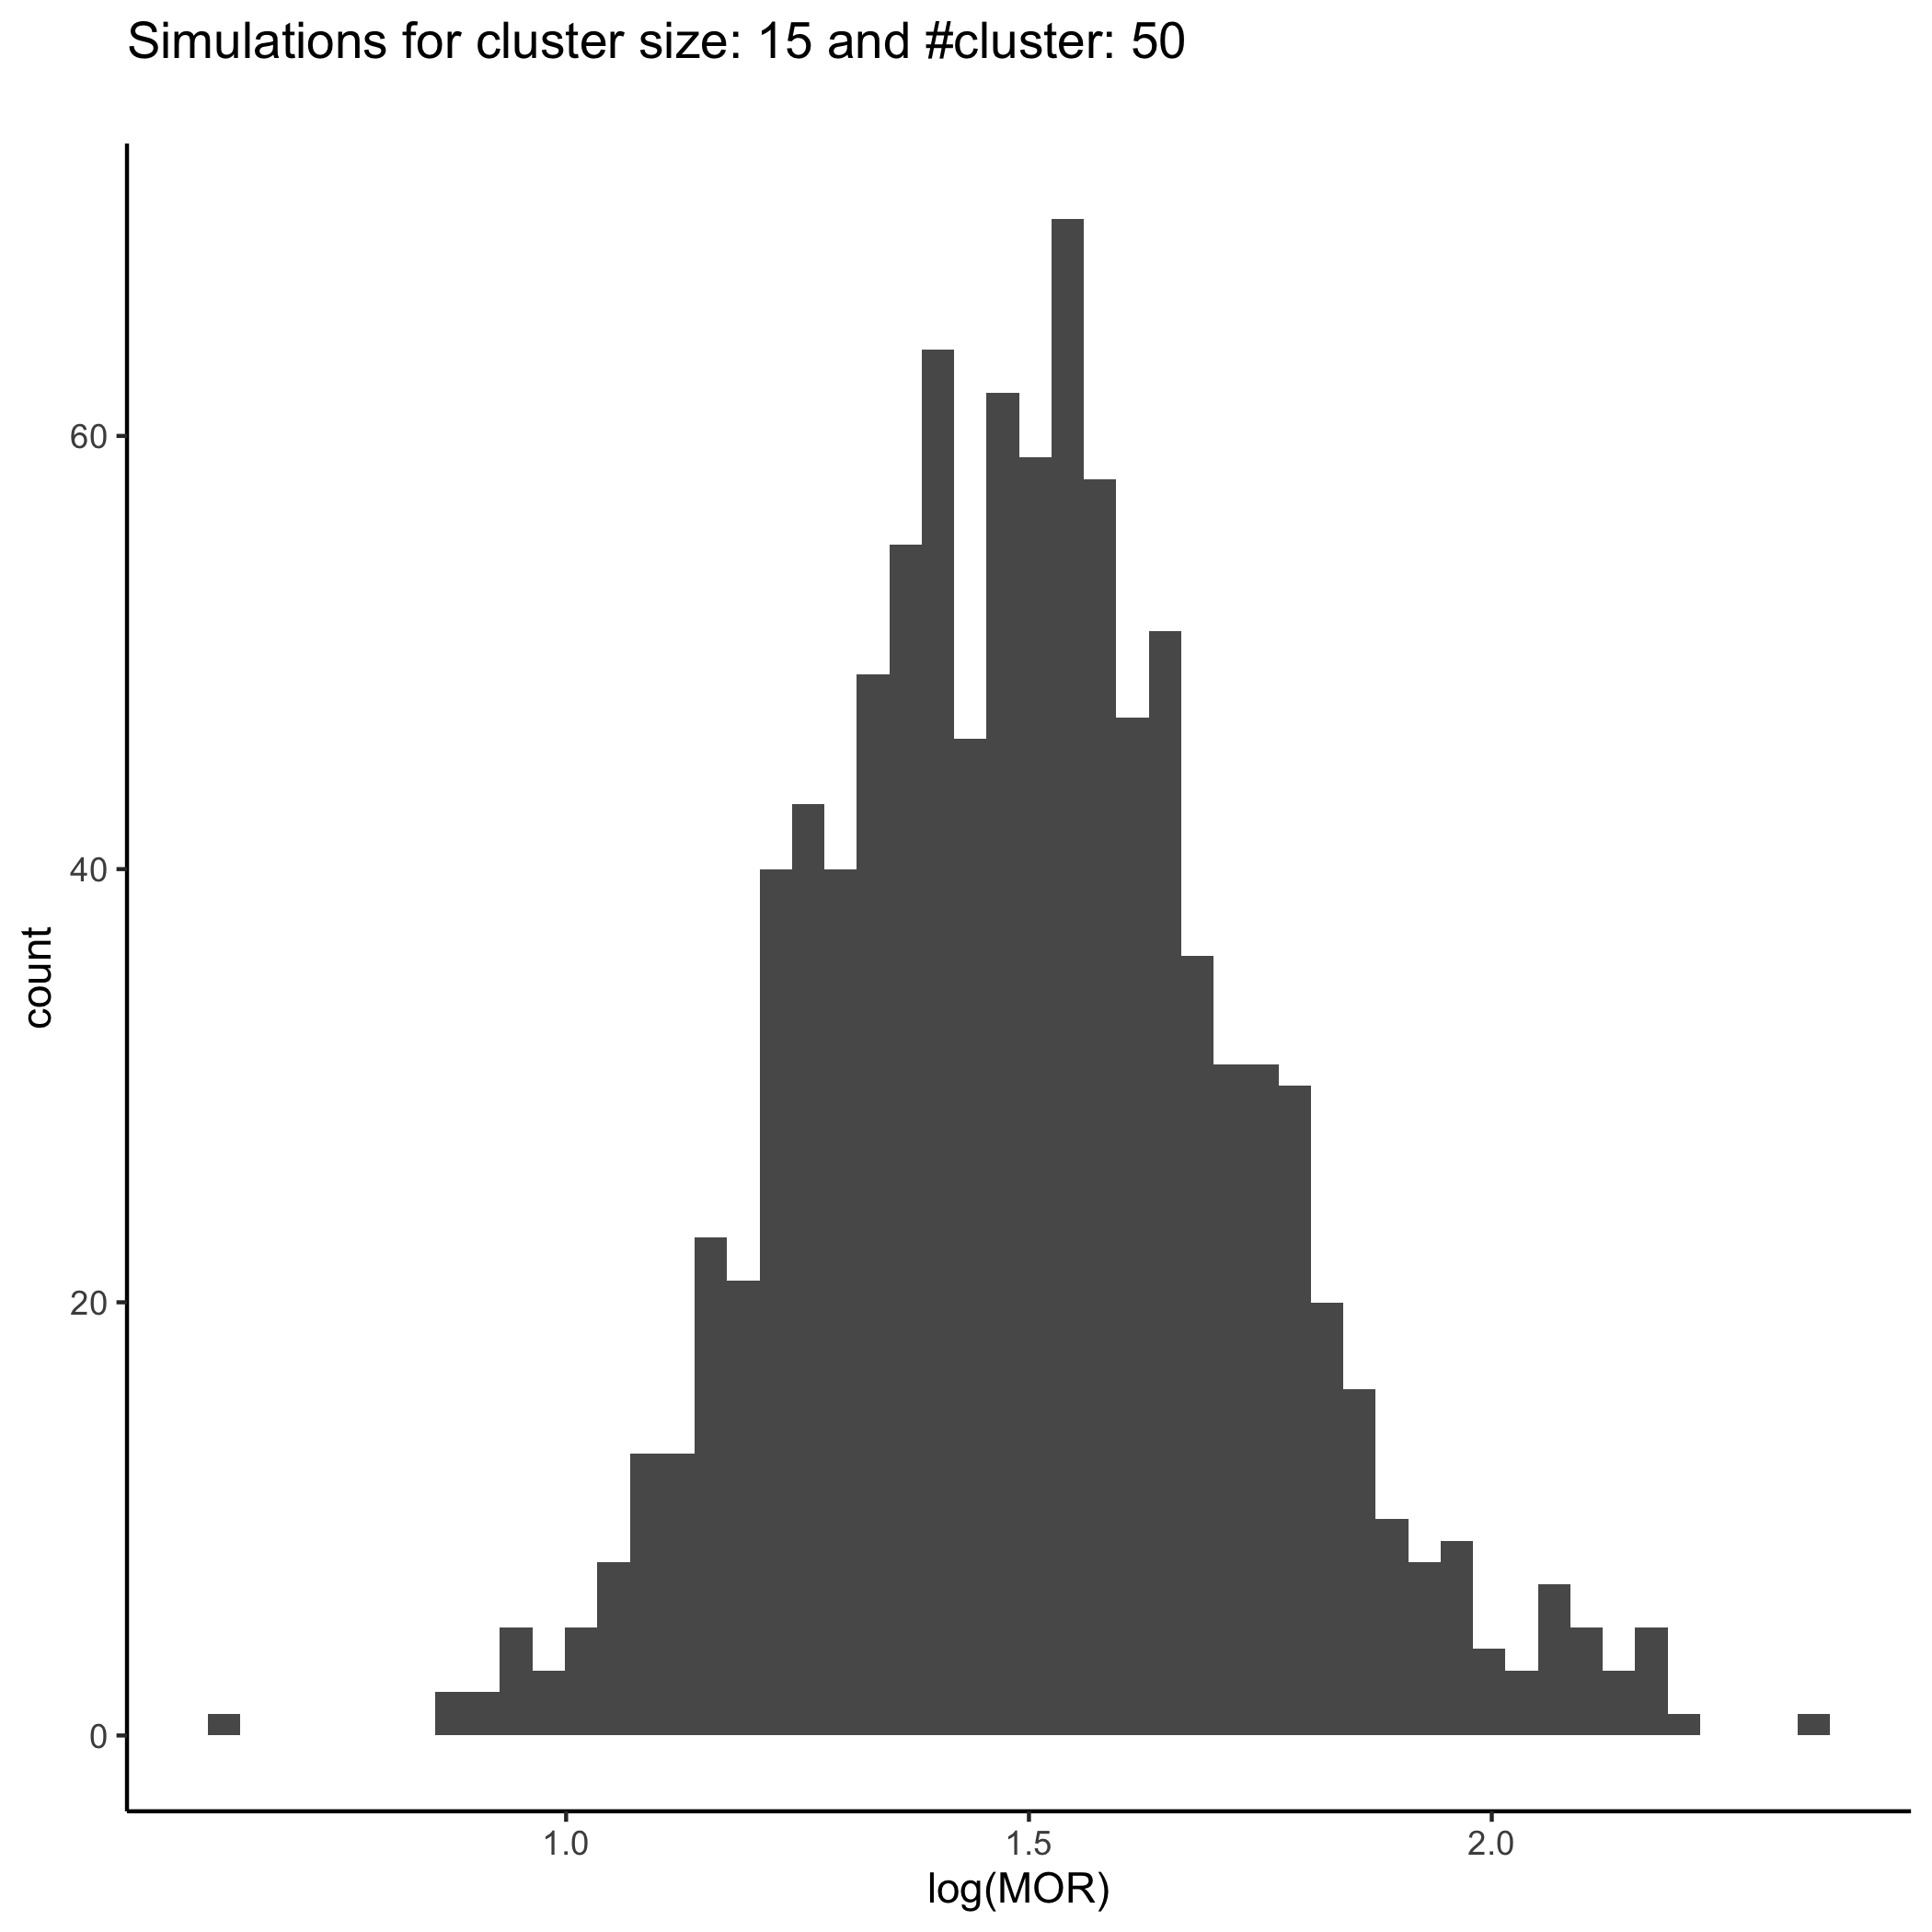
\includegraphics[width=0.5\textwidth,height=\textheight]{../plots/hist_50_15.png}

}

\caption{For 50 clusters when each of the cluster size is 15}

\end{figure}

\newpage

\hypertarget{histograms-for-logwidehatmor-when-cluster-size-is-30}{%
\section{\texorpdfstring{Histograms for \(log(\widehat{MOR})\) When
Cluster Size is
30}{Histograms for log(\textbackslash widehat\{MOR\}) When Cluster Size is 30}}\label{histograms-for-logwidehatmor-when-cluster-size-is-30}}

\vspace{5mm}

\begin{figure}

\begin{minipage}[t]{0.44\linewidth}

{\centering 

\raisebox{-\height}{

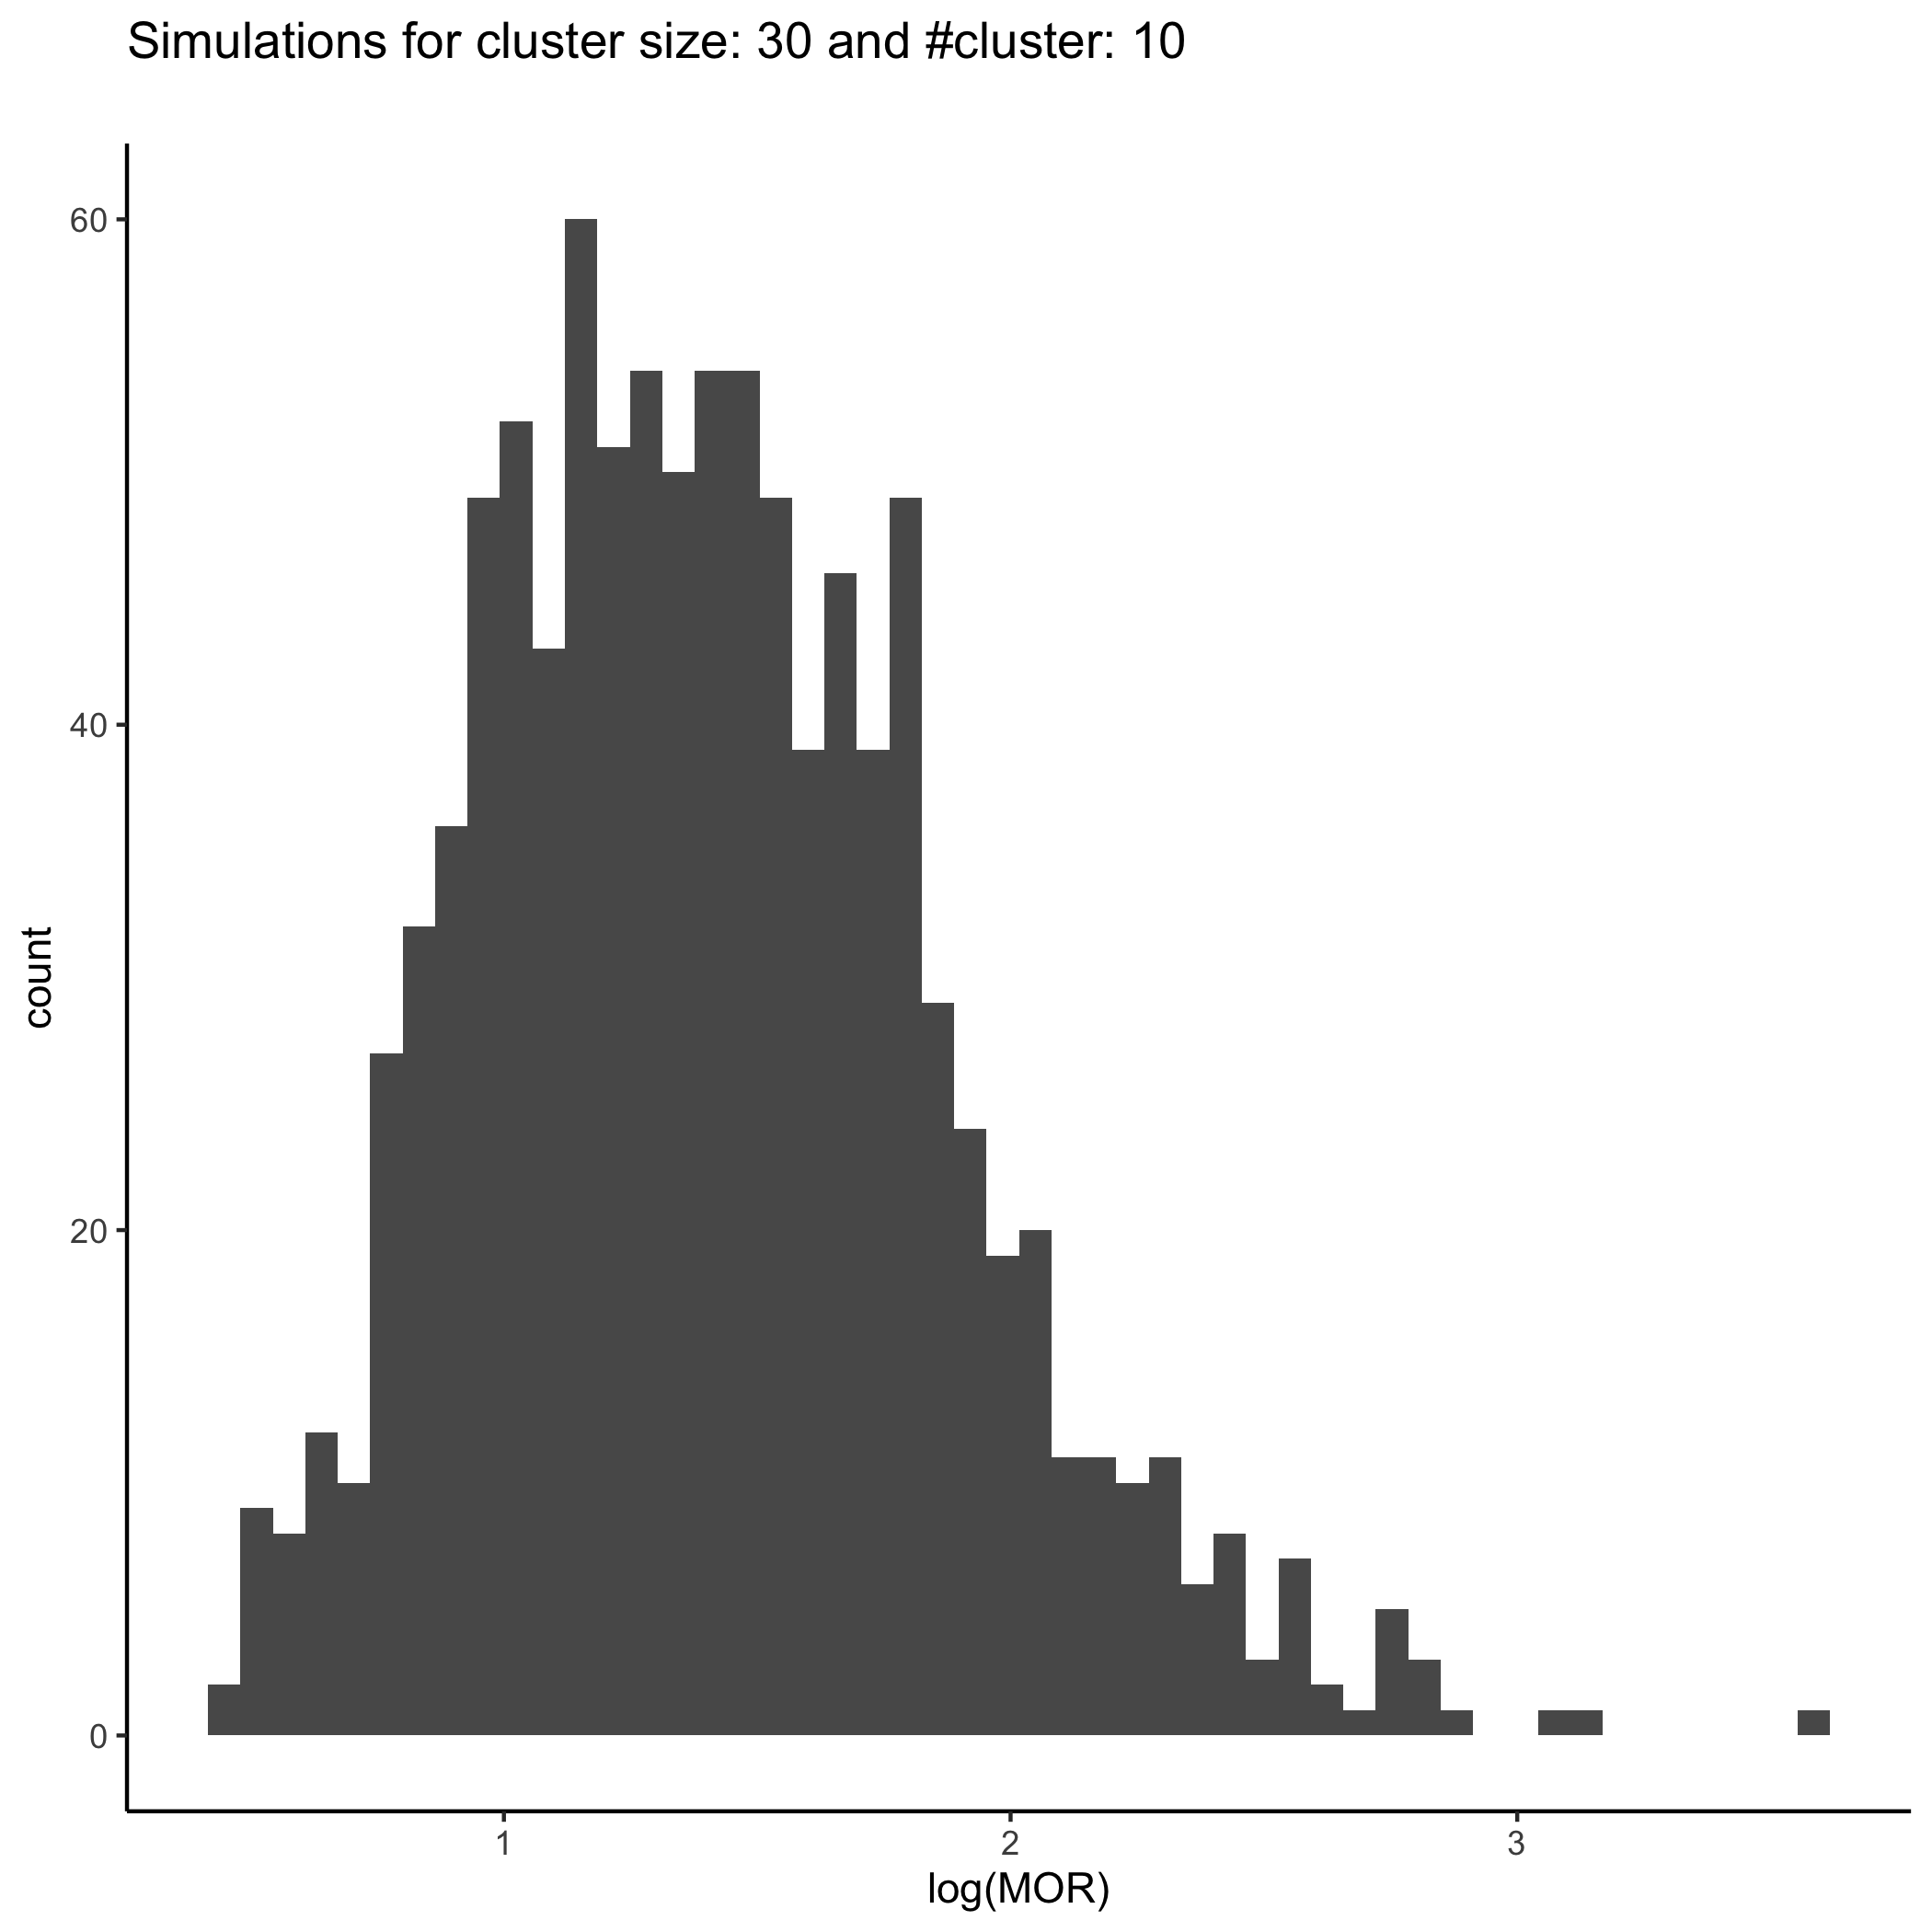
\includegraphics{../plots/hist_10_30.png}

}

\caption{For 10 clusters when each of the cluster size is 30}

}

\end{minipage}%
%
\begin{minipage}[t]{0.11\linewidth}

{\centering 

~

}

\end{minipage}%
%
\begin{minipage}[t]{0.44\linewidth}

{\centering 

\raisebox{-\height}{

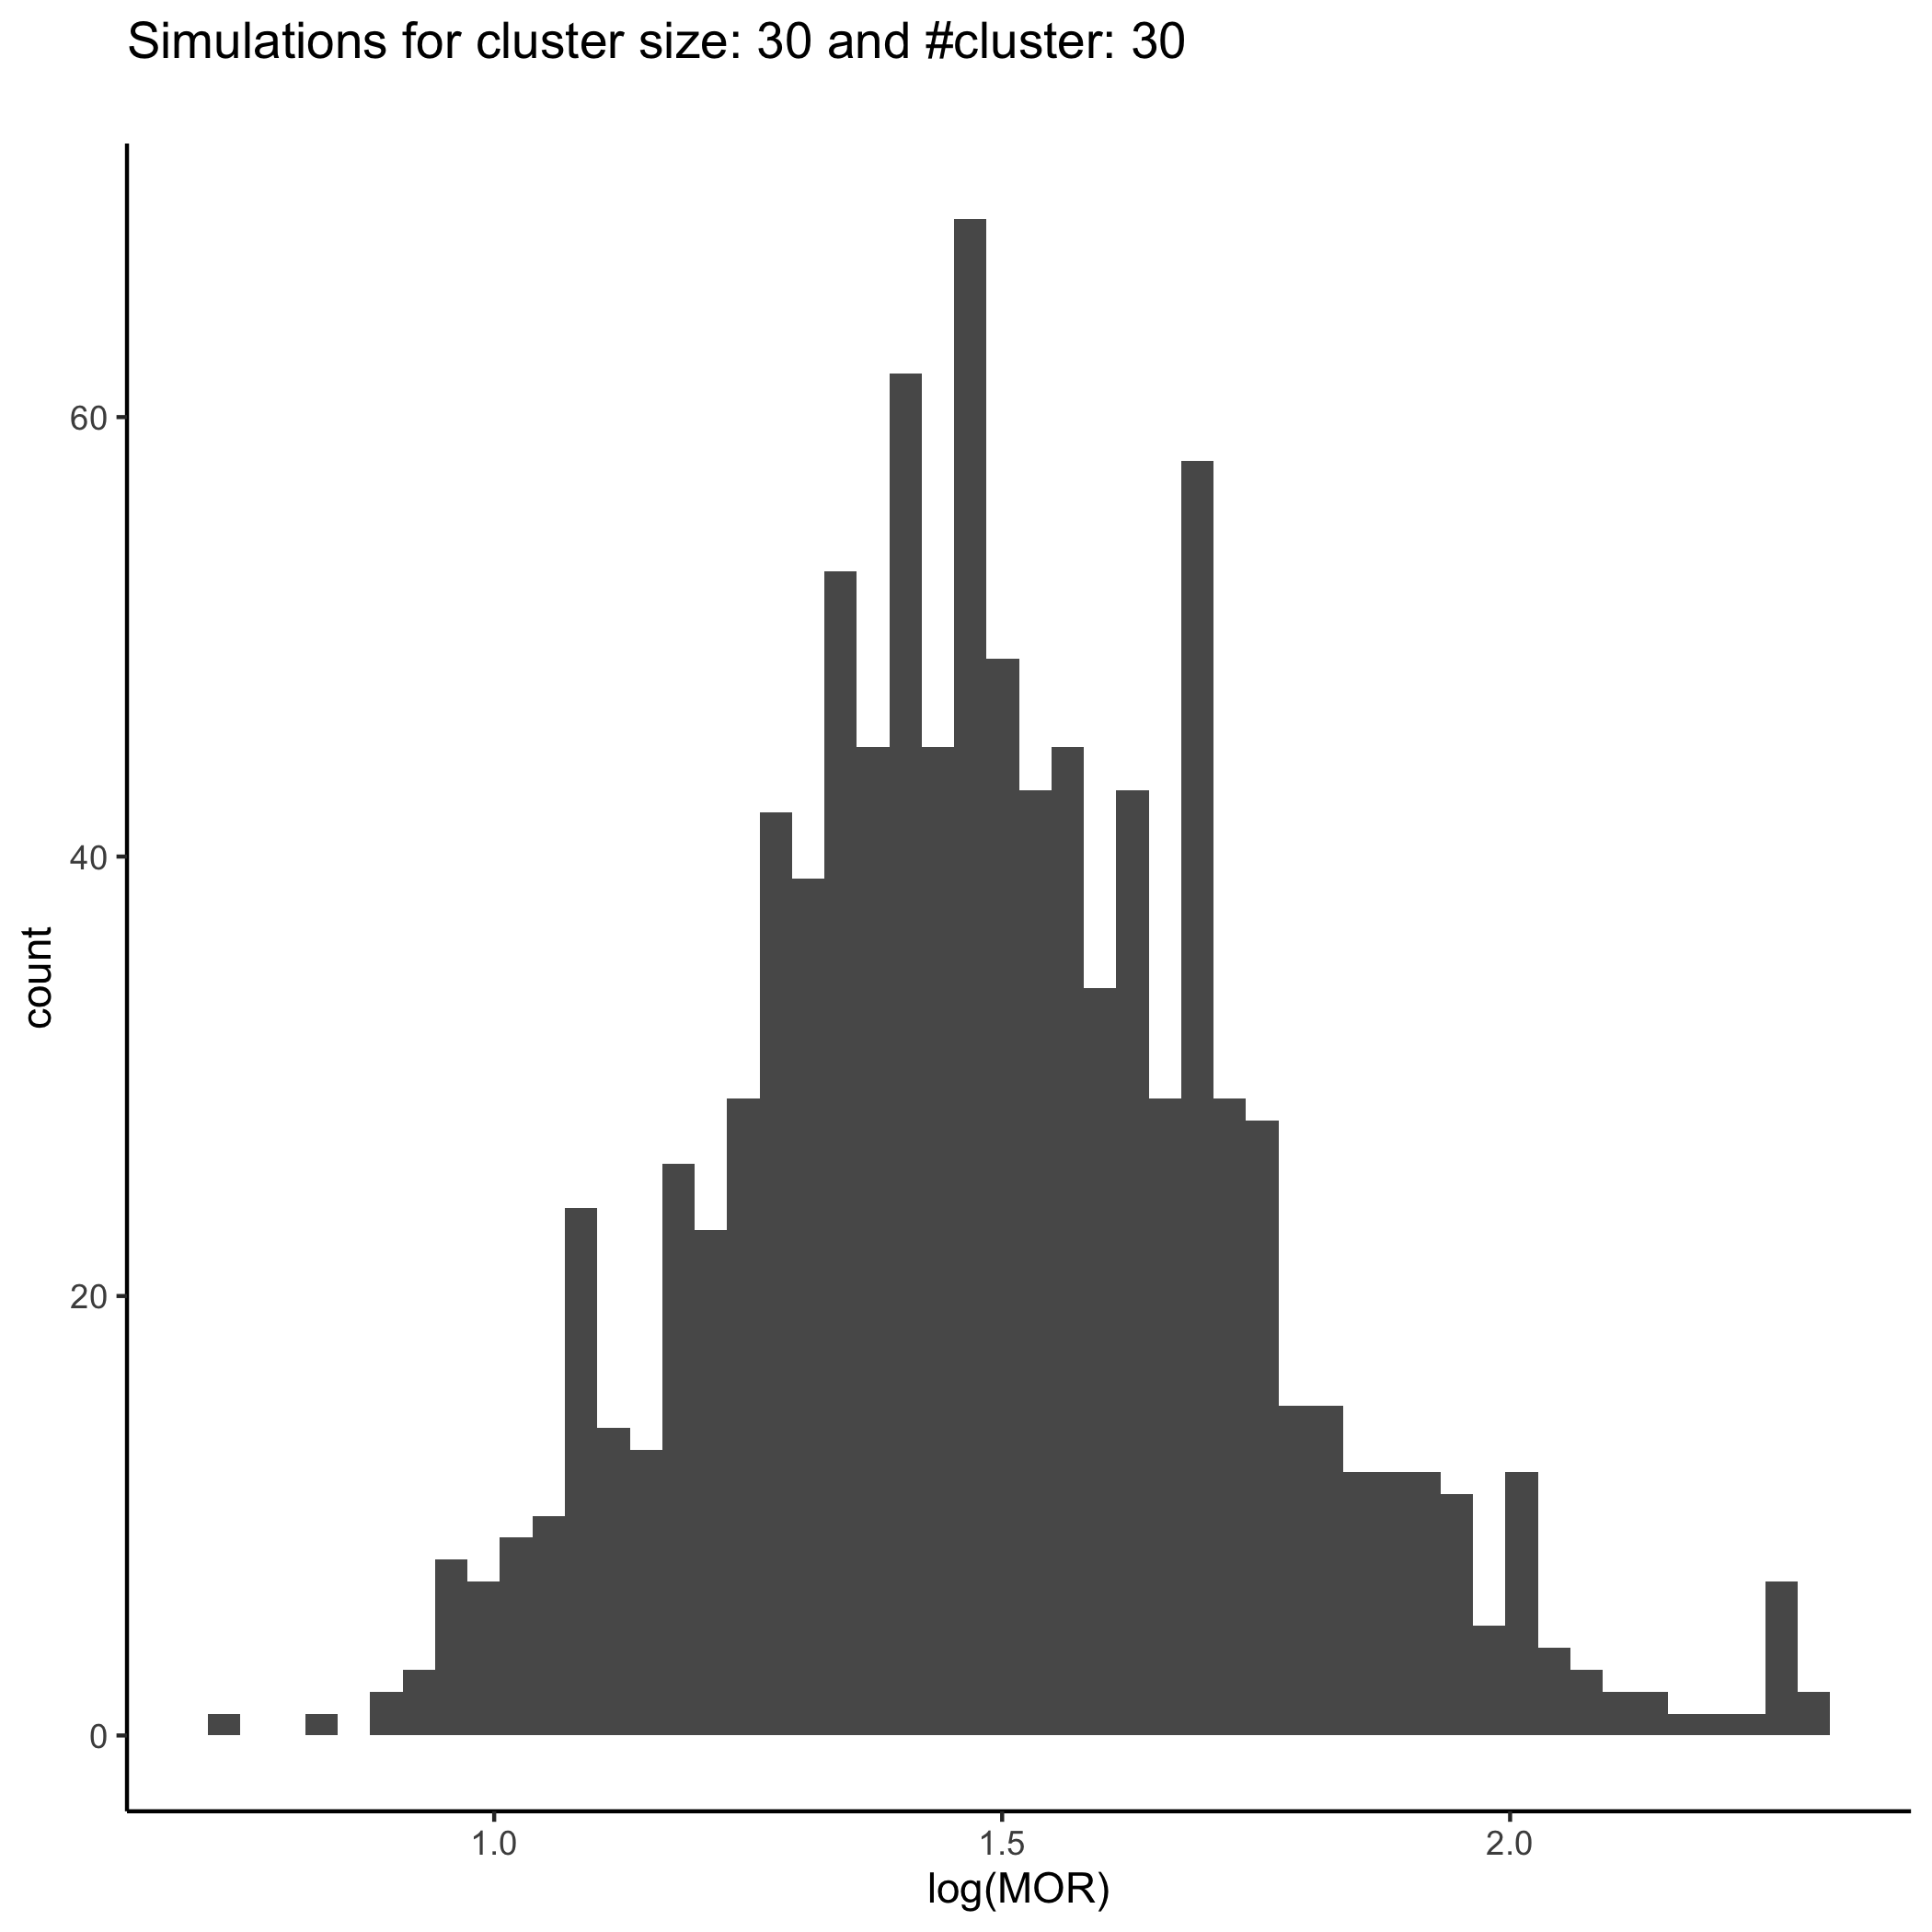
\includegraphics{../plots/hist_30_30.png}

}

\caption{For 30 clusters when each of the cluster size is 30}

}

\end{minipage}%

\end{figure}

\vspace{5mm}

\begin{figure}[H]

{\centering 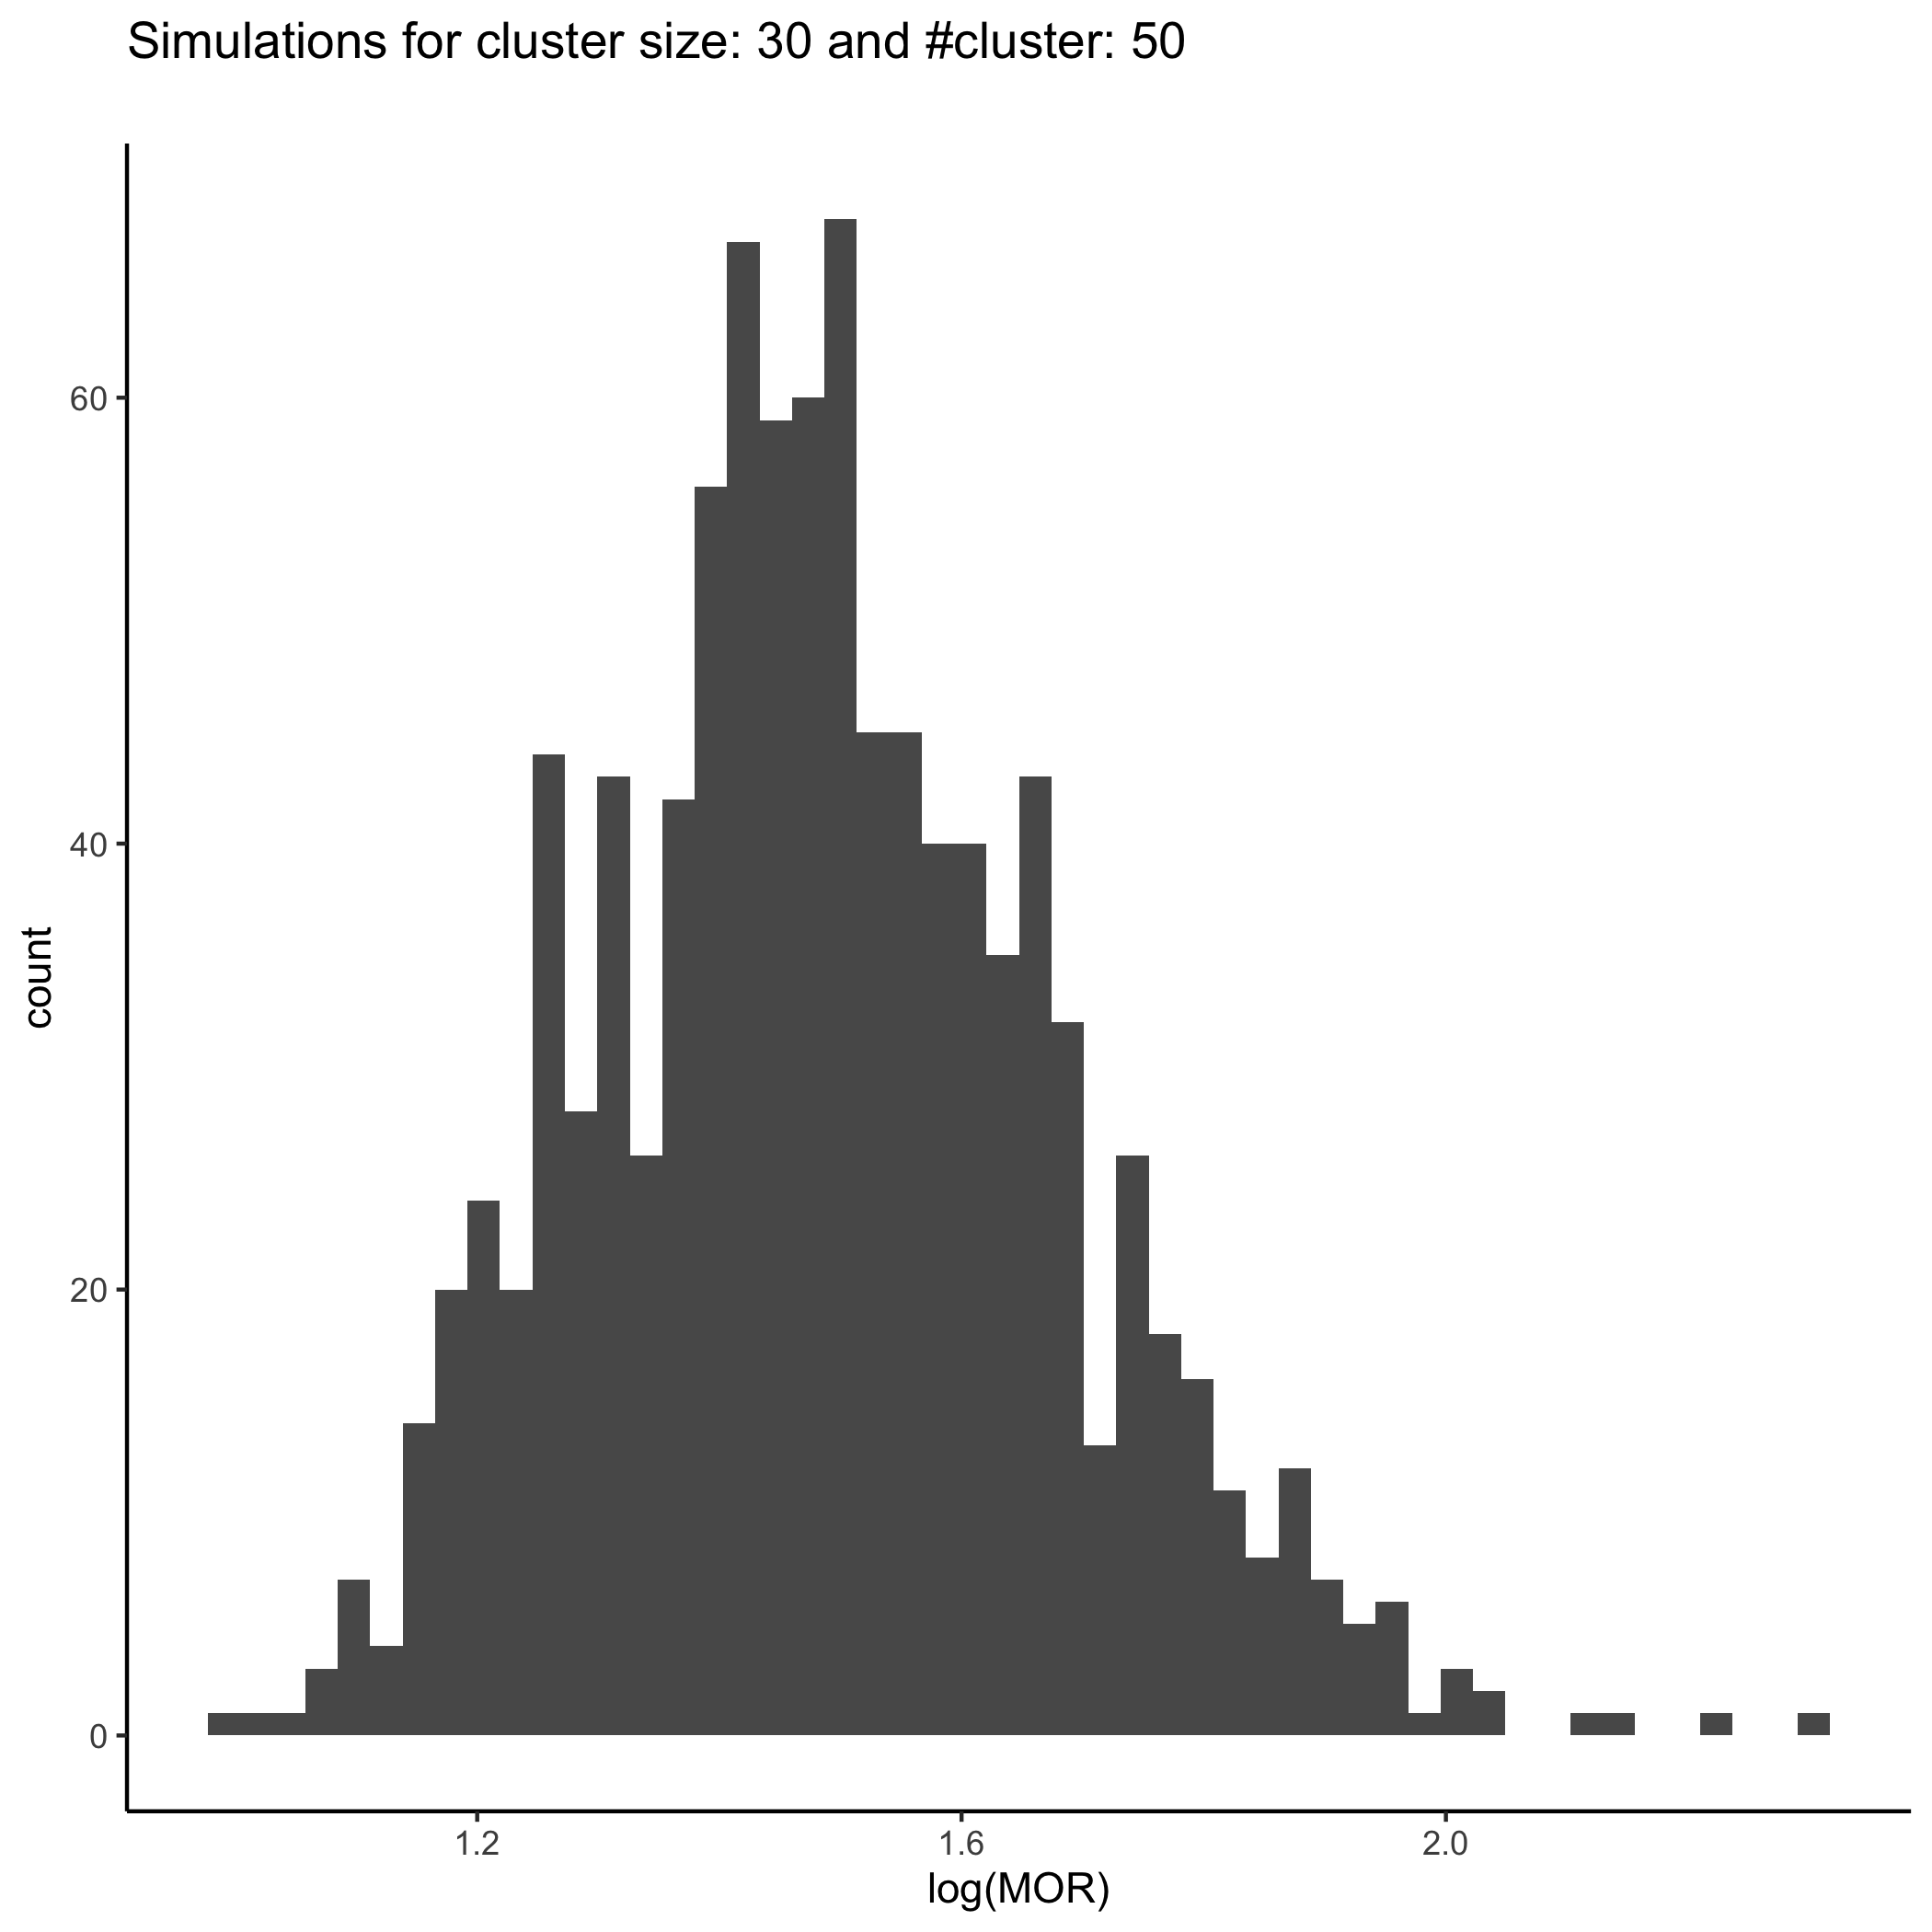
\includegraphics[width=0.5\textwidth,height=\textheight]{../plots/hist_50_30.png}

}

\caption{For 50 clusters when each of the cluster size is 30}

\end{figure}

\newpage

\hypertarget{histograms-for-logwidehatmor-when-cluster-size-is-50}{%
\section{\texorpdfstring{Histograms for \(log(\widehat{MOR})\) When
Cluster Size is
50}{Histograms for log(\textbackslash widehat\{MOR\}) When Cluster Size is 50}}\label{histograms-for-logwidehatmor-when-cluster-size-is-50}}

\vspace{5mm}

\begin{figure}

\begin{minipage}[t]{0.44\linewidth}

{\centering 

\raisebox{-\height}{

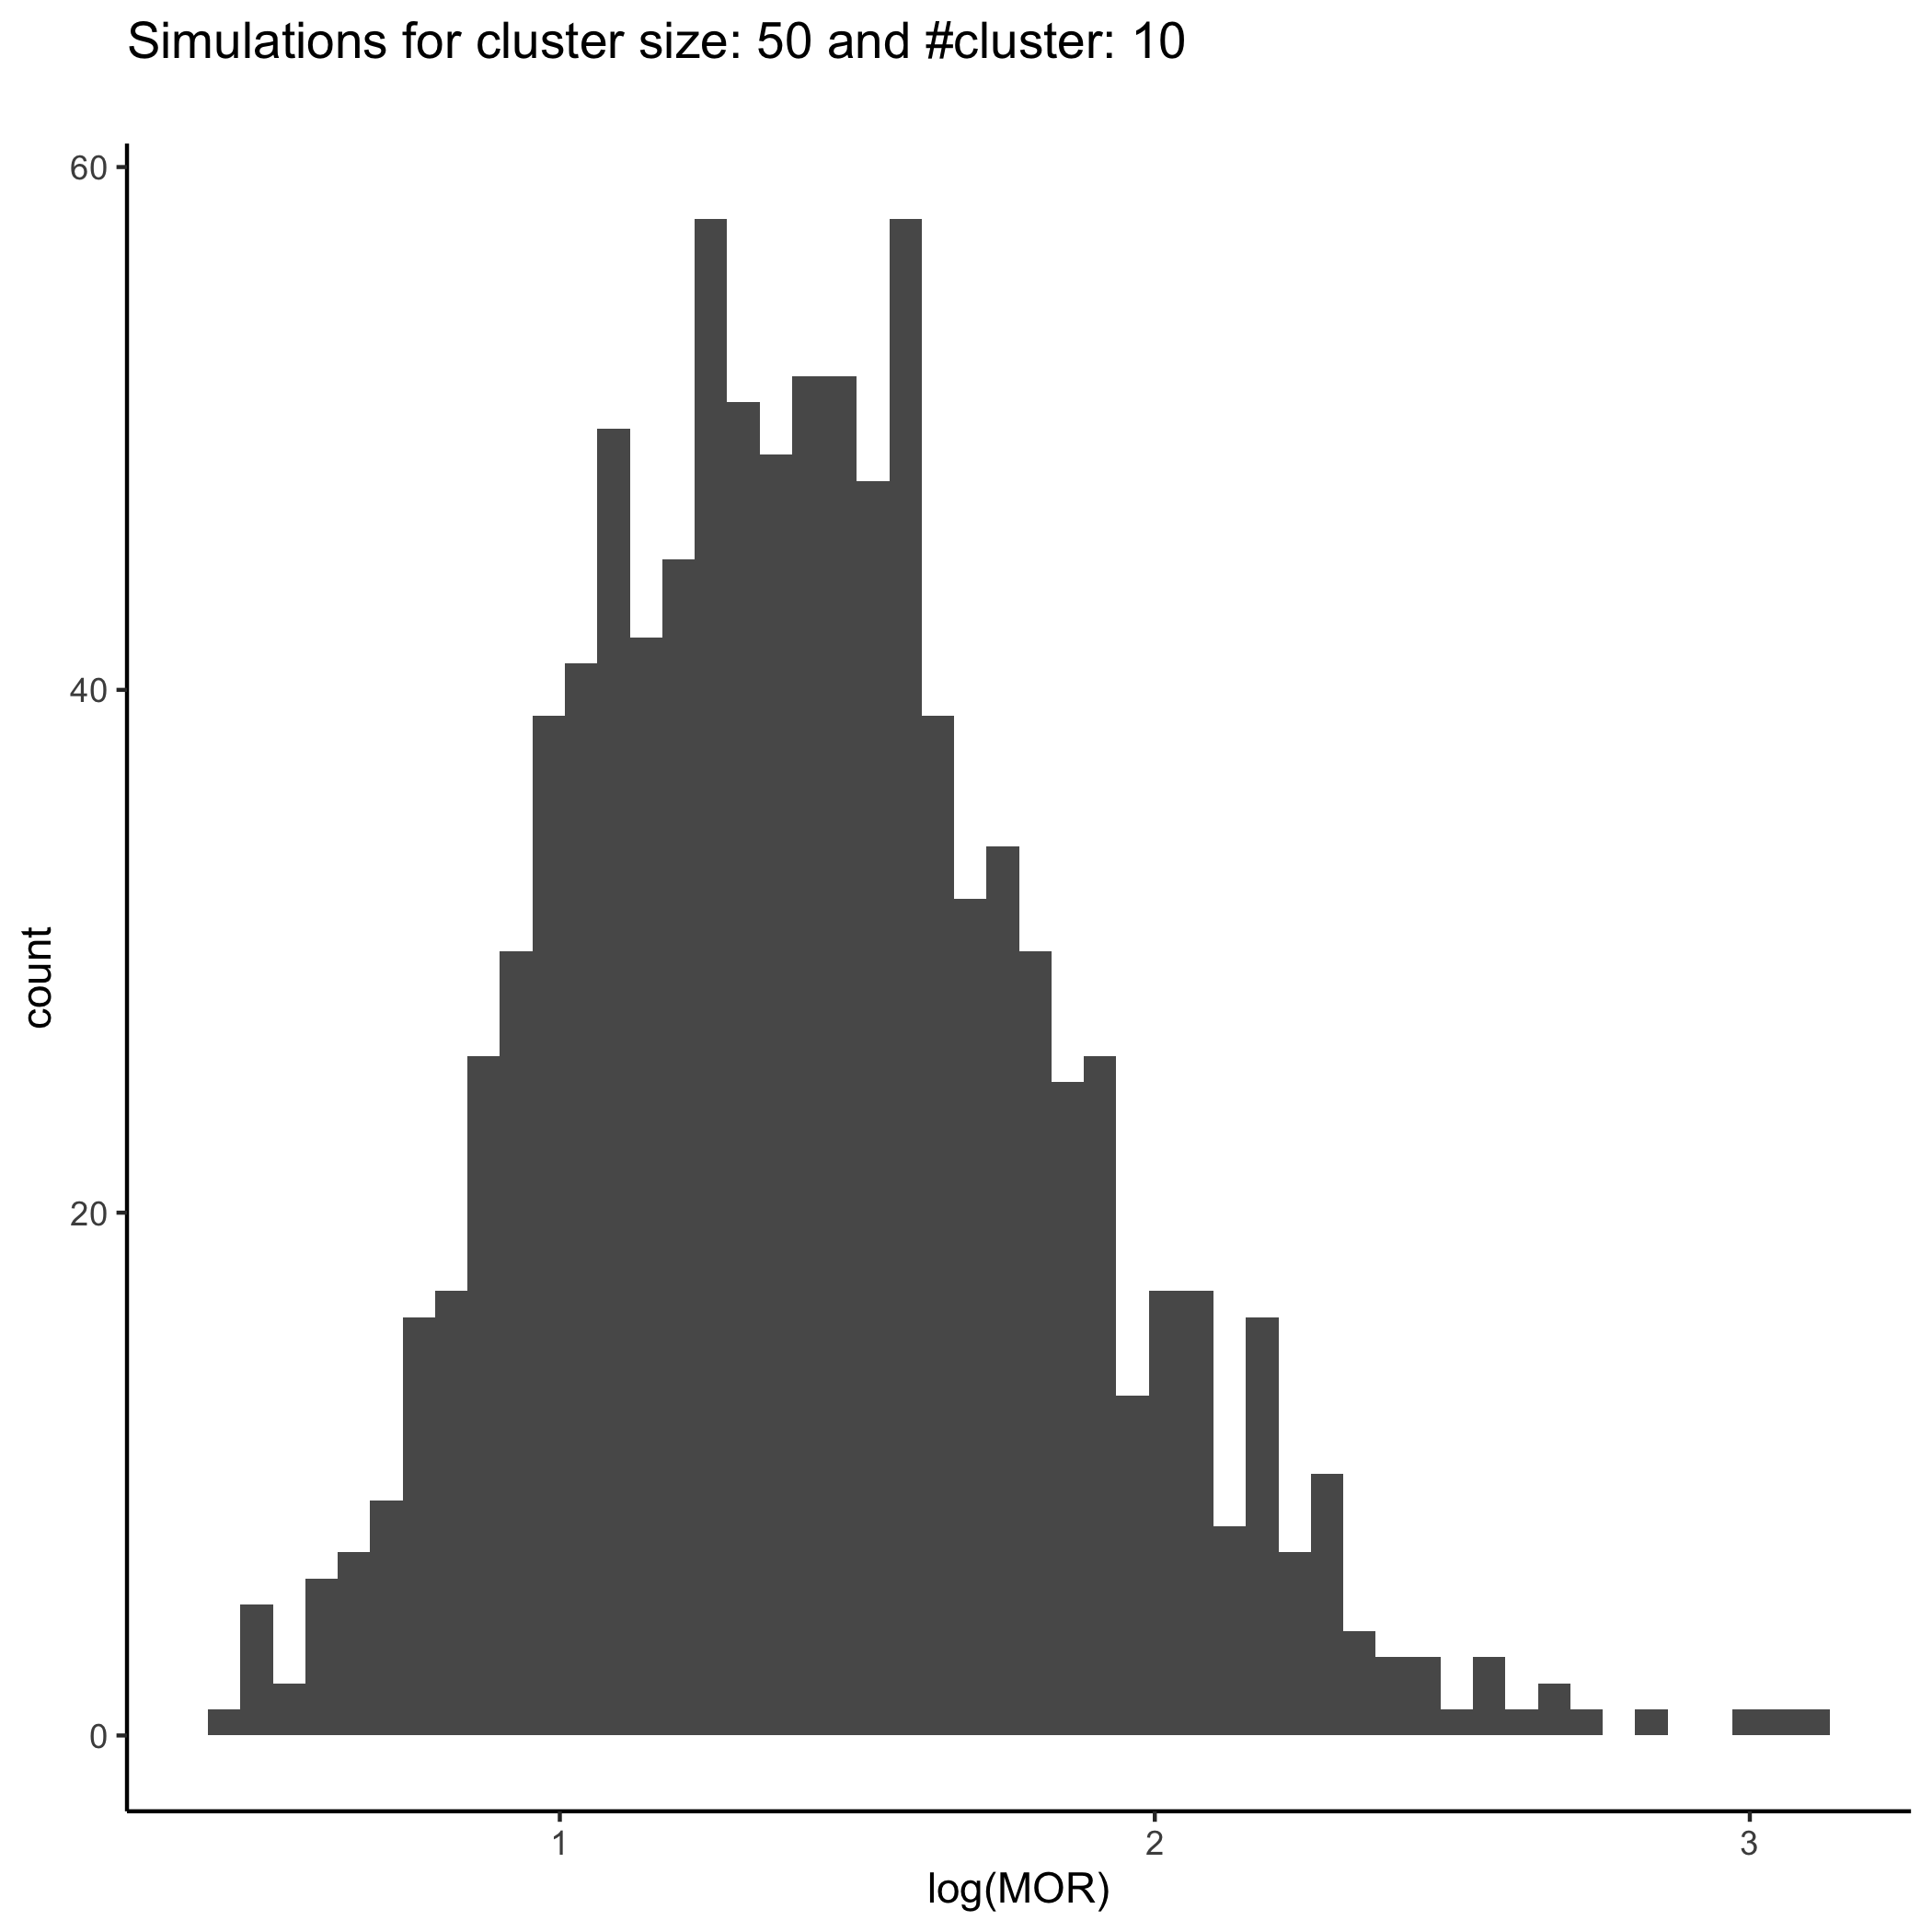
\includegraphics{../plots/hist_10_50.png}

}

\caption{For 10 clusters when each of the cluster size is 50}

}

\end{minipage}%
%
\begin{minipage}[t]{0.11\linewidth}

{\centering 

~

}

\end{minipage}%
%
\begin{minipage}[t]{0.44\linewidth}

{\centering 

\raisebox{-\height}{

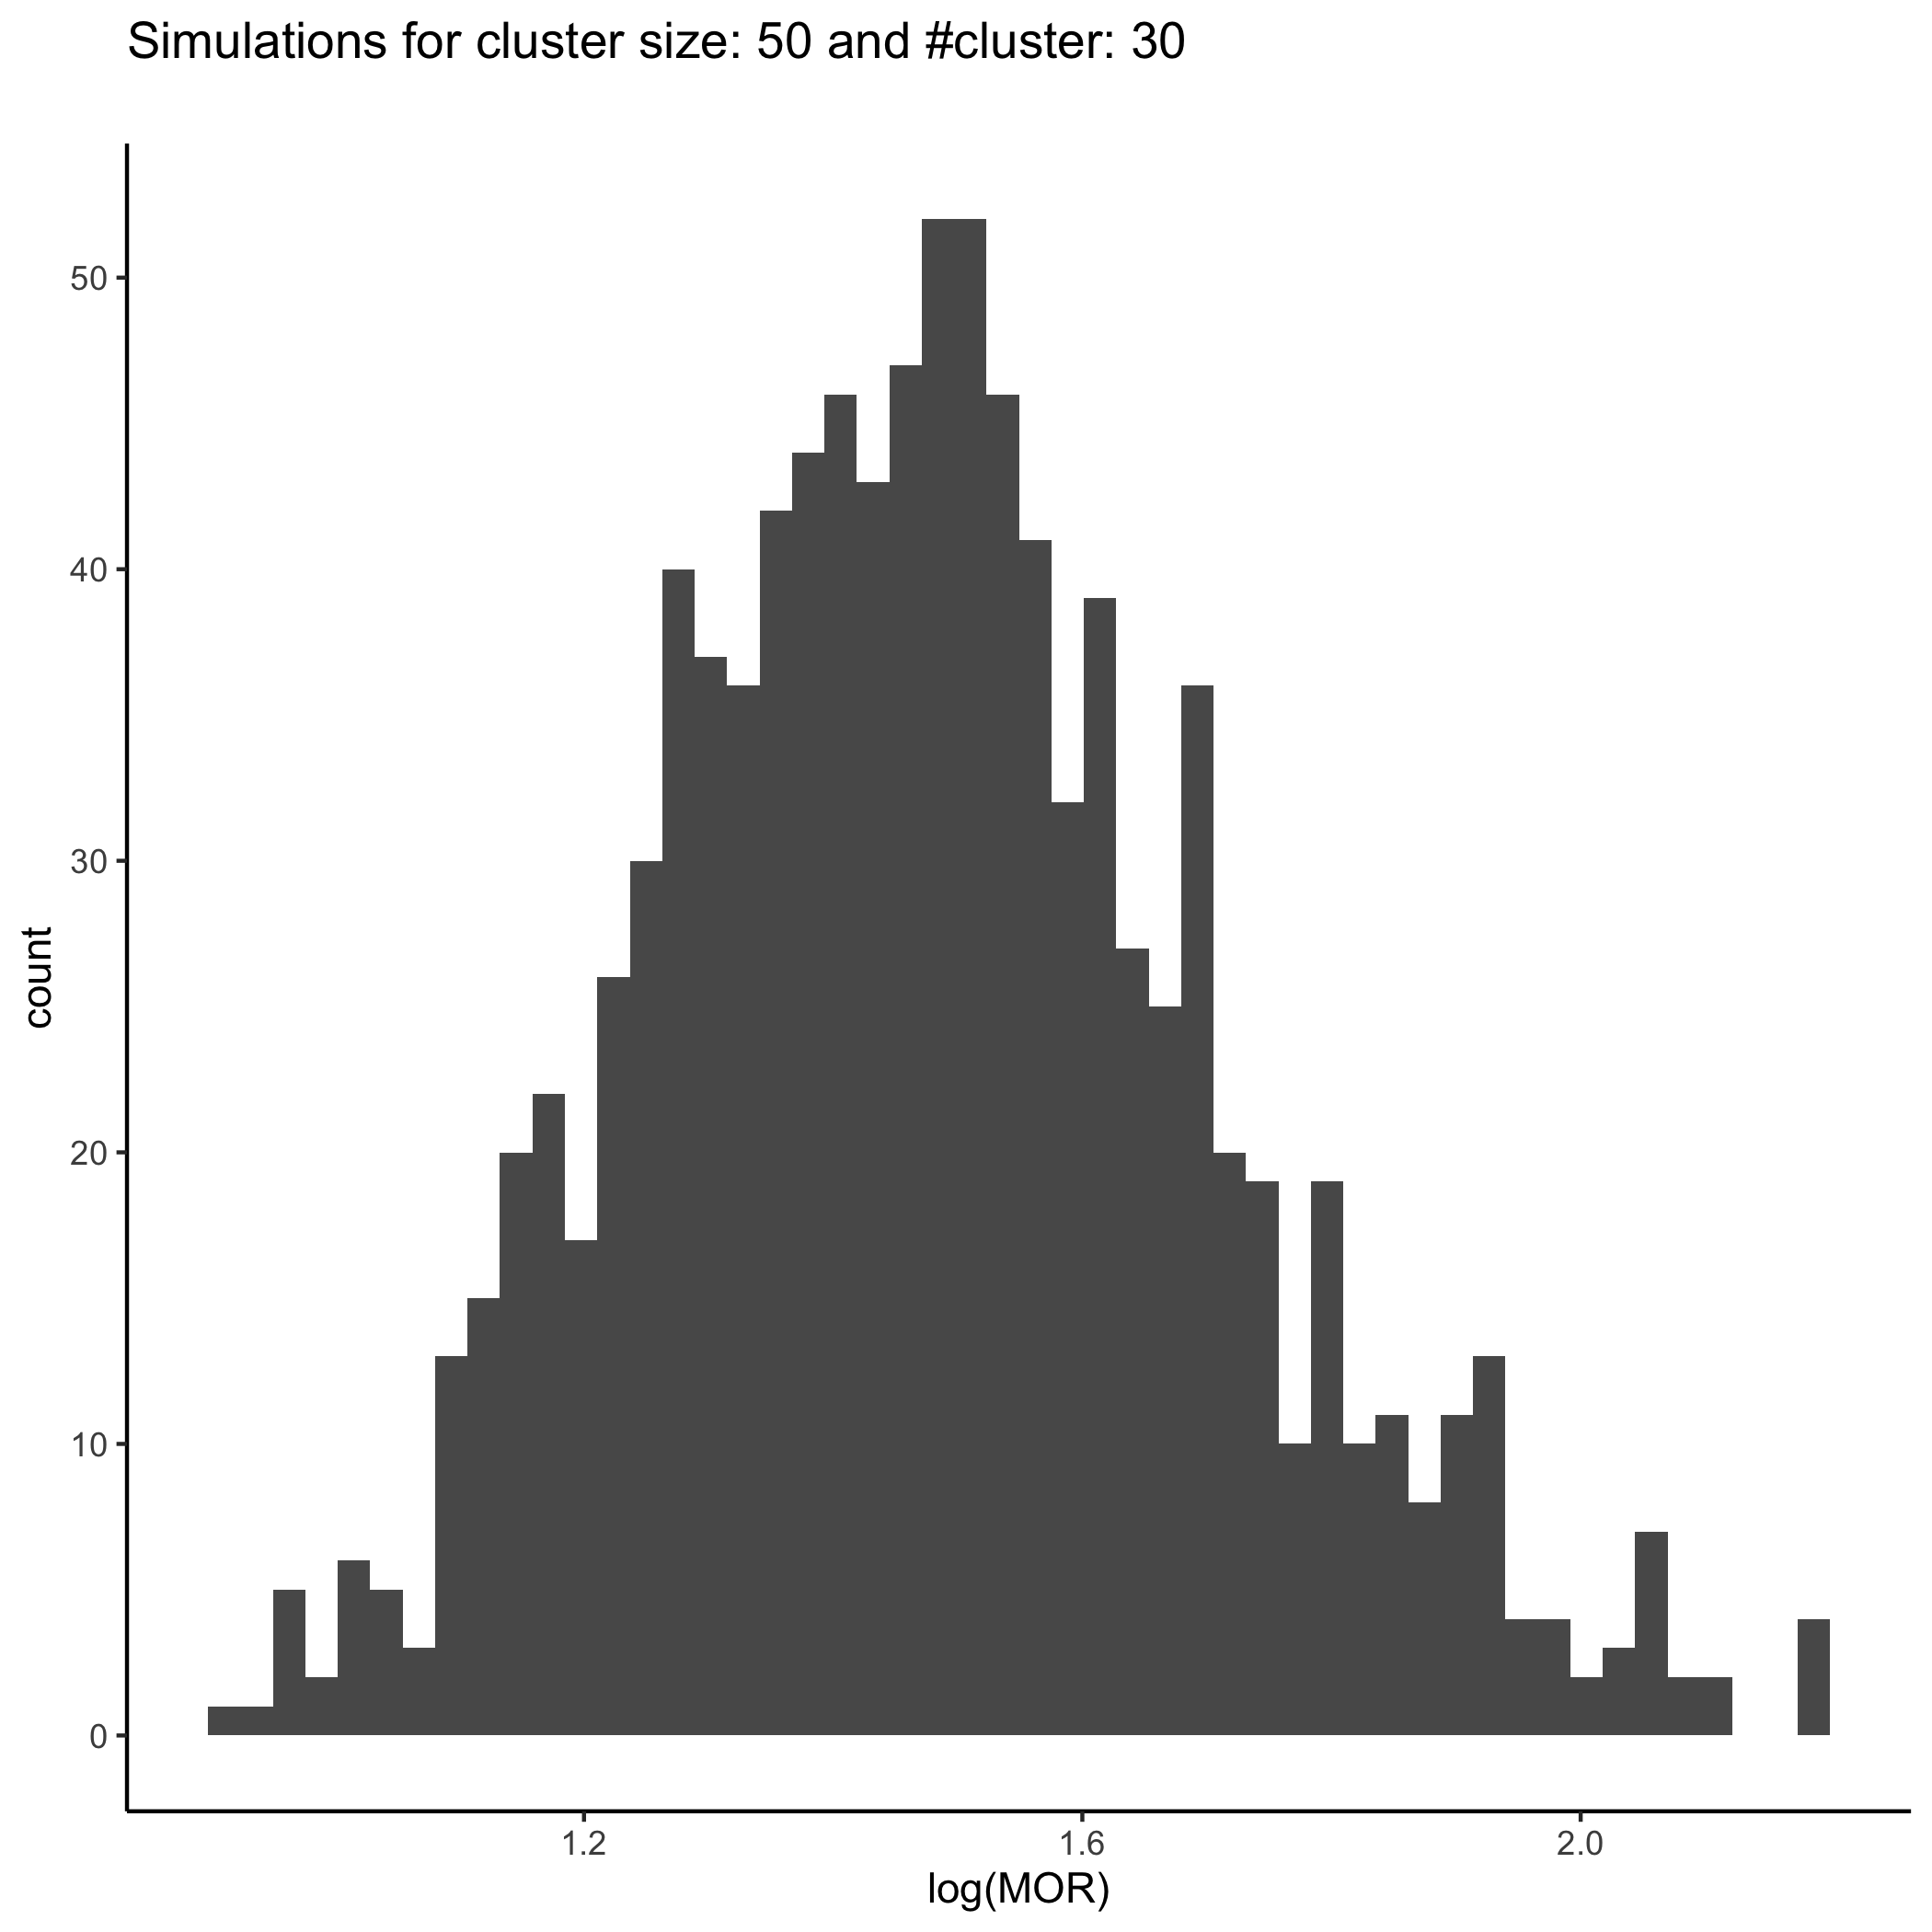
\includegraphics{../plots/hist_30_50.png}

}

\caption{For 30 clusters when each of the cluster size is 50}

}

\end{minipage}%

\end{figure}

\vspace{5mm}

\begin{figure}[H]

{\centering 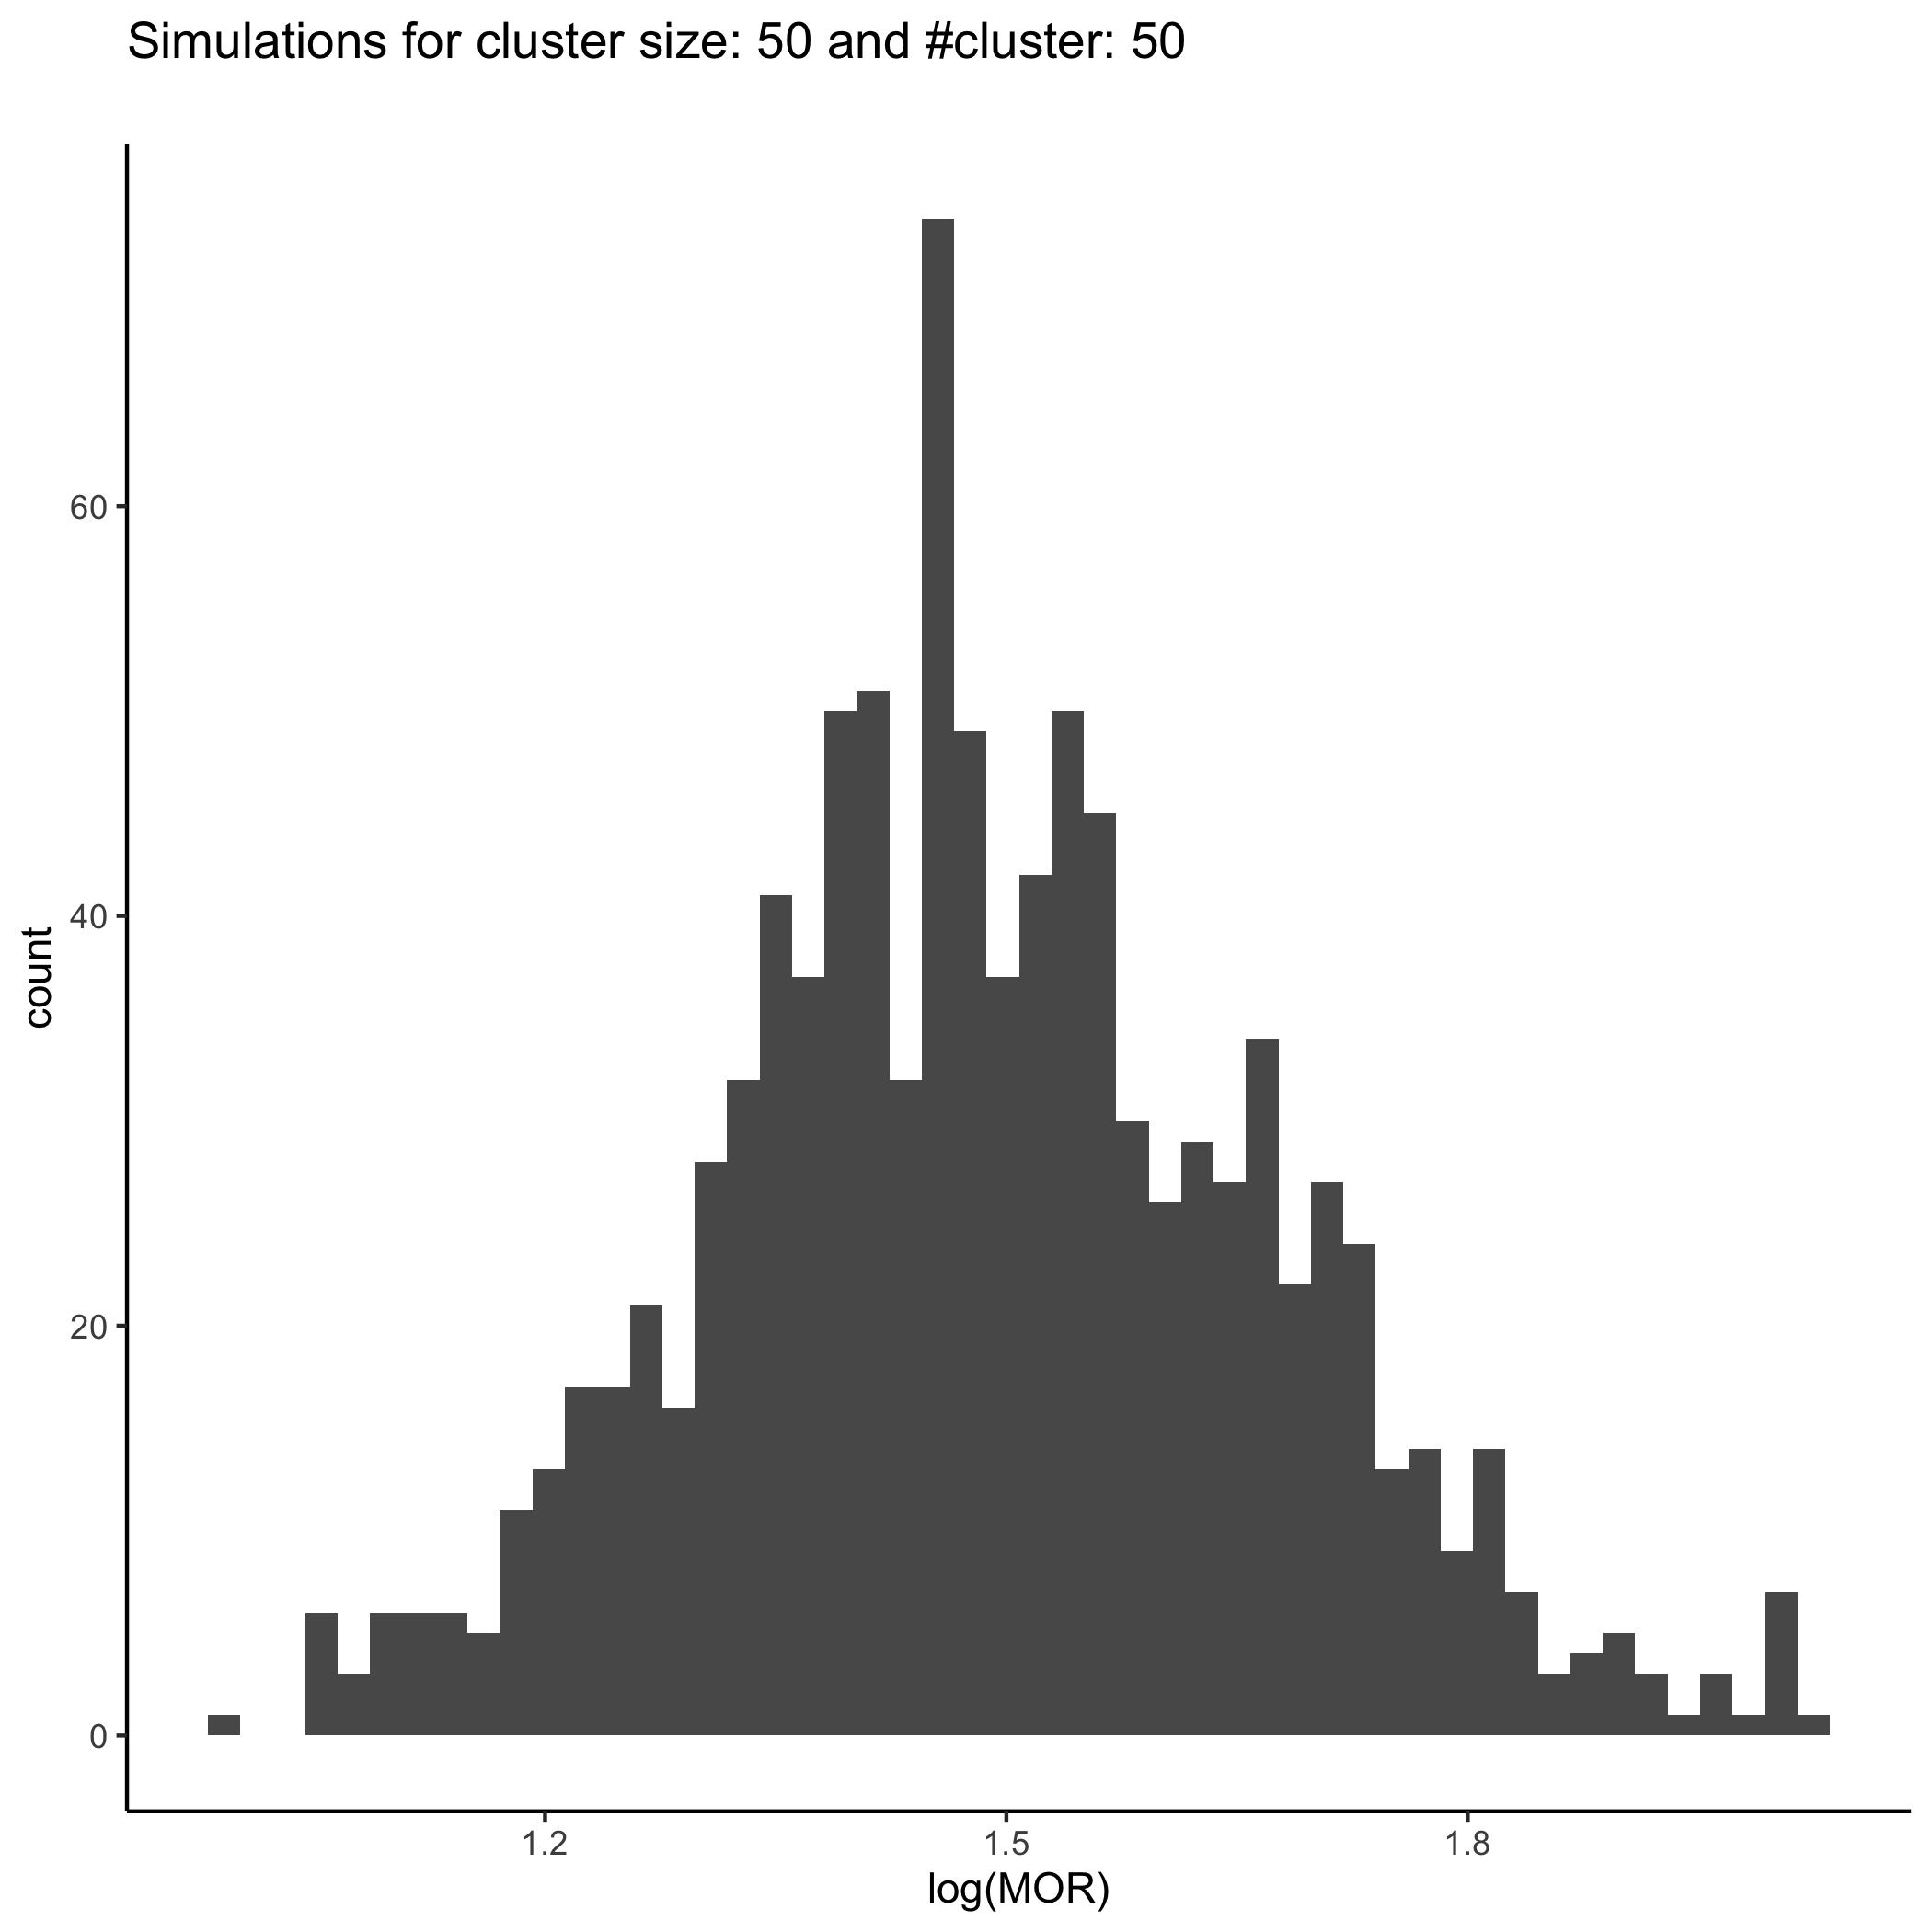
\includegraphics[width=0.5\textwidth,height=\textheight]{../plots/hist_50_50.png}

}

\caption{For 50 clusters when each of the cluster size is 50}

\end{figure}

\vspace{10mm}

\textbf{Note: 50 bins were used to create these histograms}

\newpage

\KOMAoptions{usegeometry,paper=landscape,pagesize}
\recalctypearea
\newgeometry{right=10mm,left=20mm}

\hypertarget{simulation-result-table}{%
\section{Simulation Result Table}\label{simulation-result-table}}

\begingroup

\fontsize{12pt}{18pt}\selectfont
\addtolength{\tabcolsep}{-2pt}

\begin{tabular}[t]{ccccccccccccc}
\toprule
m & n & $\widehat{MOR}$ & $\widehat{SE}(MOR)$ & $\widehat{\sigma_u^2}$ & $\widehat{\beta_0}$ & $\widehat{\beta_1}$ & $\widehat{\beta_2}$ & CI\_coverage & $Sim\_\widehat{SE(MOR)}$ & Relative Bias (\%) & Problems & Runs used\\
\midrule
10 & 10 & 688.751 & 136.147 & 3.332 & 2.117 & 1.867 & 0.759 & 0.926 & 21471.659 & 15142.532 & 0.049 & 951\\
30 & 10 & 4.854 & 1.453 & 2.639 & 2.054 & 1.785 & 0.704 & 0.950 & 2.123 & 7.421 & 0.000 & 1000\\
50 & 10 & 4.743 & 1.329 & 2.607 & 2.040 & 1.784 & 0.687 & 0.940 & 1.520 & 4.959 & 0.000 & 1000\\
10 & 15 & 5.341 & 1.946 & 2.731 & 2.070 & 1.829 & 0.707 & 0.901 & 5.295 & 18.191 & 0.008 & 992\\
30 & 15 & 4.644 & 1.366 & 2.529 & 2.029 & 1.781 & 0.692 & 0.925 & 1.611 & 2.767 & 0.000 & 1000\\
\addlinespace
50 & 15 & 4.596 & 1.271 & 2.524 & 2.018 & 1.766 & 0.677 & 0.949 & 1.132 & 1.715 & 0.000 & 1000\\
10 & 30 & 4.666 & 1.562 & 2.456 & 2.021 & 1.773 & 0.708 & 0.876 & 2.757 & 3.272 & 0.001 & 999\\
30 & 30 & 4.581 & 1.292 & 2.507 & 2.023 & 1.763 & 0.674 & 0.920 & 1.233 & 1.371 & 0.000 & 1000\\
50 & 30 & 4.525 & 1.219 & 2.483 & 2.018 & 1.757 & 0.658 & 0.947 & 0.917 & 0.146 & 0.000 & 1000\\
10 & 50 & 4.556 & 1.489 & 2.417 & 2.024 & 1.777 & 0.687 & 0.873 & 2.246 & 0.832 & 0.000 & 1000\\
\addlinespace
30 & 50 & 4.505 & 1.261 & 2.460 & 2.024 & 1.755 & 0.679 & 0.929 & 1.065 & -0.305 & 0.000 & 1000\\
50 & 50 & 4.506 & 1.198 & 2.475 & 2.029 & 1.750 & 0.660 & 0.946 & 0.772 & -0.270 & 0.000 & 1000\\
\bottomrule
\end{tabular}

\endgroup

\vspace{10mm}

Here,

\begin{itemize}
\tightlist
\item
  True \(MOR\) is 4.52
\item
  True \(\sigma^2_u\) is 2.5
\item
  ``Problems'' column represent out of 1000 simulation runs, how many
  runs were problematic
\item
  ``Runs used'' column represent how many simulation runs were used to
  calculate the numbers in the corresponding row.
\end{itemize}

\newpage



\end{document}
